\documentclass[11pt,]{article}
\usepackage[left=1in,top=1in,right=1in,bottom=1in]{geometry}
\newcommand*{\authorfont}{\fontfamily{phv}\selectfont}
\usepackage[]{mathpazo}


  \usepackage[T1]{fontenc}
  \usepackage[utf8]{inputenc}



\usepackage{abstract}
\renewcommand{\abstractname}{}    % clear the title
\renewcommand{\absnamepos}{empty} % originally center

\renewenvironment{abstract}
 {{%
    \setlength{\leftmargin}{0mm}
    \setlength{\rightmargin}{\leftmargin}%
  }%
  \relax}
 {\endlist}

\makeatletter
\def\@maketitle{%
  \newpage
%  \null
%  \vskip 2em%
%  \begin{center}%
  \let \footnote \thanks
    {\fontsize{18}{20}\selectfont\raggedright  \setlength{\parindent}{0pt} \@title \par}%
}
%\fi
\makeatother




\setcounter{secnumdepth}{3}

\usepackage{color}
\usepackage{fancyvrb}
\newcommand{\VerbBar}{|}
\newcommand{\VERB}{\Verb[commandchars=\\\{\}]}
\DefineVerbatimEnvironment{Highlighting}{Verbatim}{commandchars=\\\{\}}
% Add ',fontsize=\small' for more characters per line
\usepackage{framed}
\definecolor{shadecolor}{RGB}{248,248,248}
\newenvironment{Shaded}{\begin{snugshade}}{\end{snugshade}}
\newcommand{\KeywordTok}[1]{\textcolor[rgb]{0.13,0.29,0.53}{\textbf{#1}}}
\newcommand{\DataTypeTok}[1]{\textcolor[rgb]{0.13,0.29,0.53}{#1}}
\newcommand{\DecValTok}[1]{\textcolor[rgb]{0.00,0.00,0.81}{#1}}
\newcommand{\BaseNTok}[1]{\textcolor[rgb]{0.00,0.00,0.81}{#1}}
\newcommand{\FloatTok}[1]{\textcolor[rgb]{0.00,0.00,0.81}{#1}}
\newcommand{\ConstantTok}[1]{\textcolor[rgb]{0.00,0.00,0.00}{#1}}
\newcommand{\CharTok}[1]{\textcolor[rgb]{0.31,0.60,0.02}{#1}}
\newcommand{\SpecialCharTok}[1]{\textcolor[rgb]{0.00,0.00,0.00}{#1}}
\newcommand{\StringTok}[1]{\textcolor[rgb]{0.31,0.60,0.02}{#1}}
\newcommand{\VerbatimStringTok}[1]{\textcolor[rgb]{0.31,0.60,0.02}{#1}}
\newcommand{\SpecialStringTok}[1]{\textcolor[rgb]{0.31,0.60,0.02}{#1}}
\newcommand{\ImportTok}[1]{#1}
\newcommand{\CommentTok}[1]{\textcolor[rgb]{0.56,0.35,0.01}{\textit{#1}}}
\newcommand{\DocumentationTok}[1]{\textcolor[rgb]{0.56,0.35,0.01}{\textbf{\textit{#1}}}}
\newcommand{\AnnotationTok}[1]{\textcolor[rgb]{0.56,0.35,0.01}{\textbf{\textit{#1}}}}
\newcommand{\CommentVarTok}[1]{\textcolor[rgb]{0.56,0.35,0.01}{\textbf{\textit{#1}}}}
\newcommand{\OtherTok}[1]{\textcolor[rgb]{0.56,0.35,0.01}{#1}}
\newcommand{\FunctionTok}[1]{\textcolor[rgb]{0.00,0.00,0.00}{#1}}
\newcommand{\VariableTok}[1]{\textcolor[rgb]{0.00,0.00,0.00}{#1}}
\newcommand{\ControlFlowTok}[1]{\textcolor[rgb]{0.13,0.29,0.53}{\textbf{#1}}}
\newcommand{\OperatorTok}[1]{\textcolor[rgb]{0.81,0.36,0.00}{\textbf{#1}}}
\newcommand{\BuiltInTok}[1]{#1}
\newcommand{\ExtensionTok}[1]{#1}
\newcommand{\PreprocessorTok}[1]{\textcolor[rgb]{0.56,0.35,0.01}{\textit{#1}}}
\newcommand{\AttributeTok}[1]{\textcolor[rgb]{0.77,0.63,0.00}{#1}}
\newcommand{\RegionMarkerTok}[1]{#1}
\newcommand{\InformationTok}[1]{\textcolor[rgb]{0.56,0.35,0.01}{\textbf{\textit{#1}}}}
\newcommand{\WarningTok}[1]{\textcolor[rgb]{0.56,0.35,0.01}{\textbf{\textit{#1}}}}
\newcommand{\AlertTok}[1]{\textcolor[rgb]{0.94,0.16,0.16}{#1}}
\newcommand{\ErrorTok}[1]{\textcolor[rgb]{0.64,0.00,0.00}{\textbf{#1}}}
\newcommand{\NormalTok}[1]{#1}

\usepackage{graphicx,grffile}
\makeatletter
\def\maxwidth{\ifdim\Gin@nat@width>\linewidth\linewidth\else\Gin@nat@width\fi}
\def\maxheight{\ifdim\Gin@nat@height>\textheight\textheight\else\Gin@nat@height\fi}
\makeatother
% Scale images if necessary, so that they will not overflow the page
% margins by default, and it is still possible to overwrite the defaults
% using explicit options in \includegraphics[width, height, ...]{}
\setkeys{Gin}{width=\maxwidth,height=\maxheight,keepaspectratio}

\title{Relación de los Centros de Refugios respecto a las viviendas construidas
con techo de zinc, la vulnerabilidad ante los fenómenos atmósfericos.  }



\author{\Large ALEIRA DEL JESUS, GRACE SORIANO, WILNELLIA FABIAN\vspace{0.05in} \newline\normalsize\emph{Estudiantes, Universidad Autónoma de Santo Domingo (UASD)}  }


\date{}

\usepackage{titlesec}

\titleformat*{\section}{\normalsize\bfseries}
\titleformat*{\subsection}{\normalsize\itshape}
\titleformat*{\subsubsection}{\normalsize\itshape}
\titleformat*{\paragraph}{\normalsize\itshape}
\titleformat*{\subparagraph}{\normalsize\itshape}

\titlespacing{\section}
{0pt}{36pt}{0pt}
\titlespacing{\subsection}
{0pt}{36pt}{0pt}
\titlespacing{\subsubsection}
{0pt}{36pt}{0pt}





\newtheorem{hypothesis}{Hypothesis}
\usepackage{setspace}

\makeatletter
\@ifpackageloaded{hyperref}{}{%
\ifxetex
  \PassOptionsToPackage{hyphens}{url}\usepackage[setpagesize=false, % page size defined by xetex
              unicode=false, % unicode breaks when used with xetex
              xetex]{hyperref}
\else
  \PassOptionsToPackage{hyphens}{url}\usepackage[unicode=true]{hyperref}
\fi
}

\@ifpackageloaded{color}{
    \PassOptionsToPackage{usenames,dvipsnames}{color}
}{%
    \usepackage[usenames,dvipsnames]{color}
}
\makeatother
\hypersetup{breaklinks=true,
            bookmarks=true,
            pdfauthor={ALEIRA DEL JESUS, GRACE SORIANO, WILNELLIA FABIAN (Estudiantes, Universidad Autónoma de Santo Domingo (UASD))},
             pdfkeywords = {Ordenamiento territorial, Fenómeno Natural},  
            pdftitle={Relación de los Centros de Refugios respecto a las viviendas construidas
con techo de zinc, la vulnerabilidad ante los fenómenos atmósfericos.},
            colorlinks=true,
            citecolor=blue,
            urlcolor=blue,
            linkcolor=magenta,
            pdfborder={0 0 0}}
\urlstyle{same}  % don't use monospace font for urls

% set default figure placement to htbp
\makeatletter
\def\fps@figure{htbp}
\makeatother

\usepackage{pdflscape} \newcommand{\blandscape}{\begin{landscape}}
\newcommand{\elandscape}{\end{landscape}}


% add tightlist ----------
\providecommand{\tightlist}{%
\setlength{\itemsep}{0pt}\setlength{\parskip}{0pt}}

\begin{document}
	
% \pagenumbering{arabic}% resets `page` counter to 1 
%
% \maketitle

{% \usefont{T1}{pnc}{m}{n}
\setlength{\parindent}{0pt}
\thispagestyle{plain}
{\fontsize{18}{20}\selectfont\raggedright 
\maketitle  % title \par  

}

{
   \vskip 13.5pt\relax \normalsize\fontsize{11}{12} 
\textbf{\authorfont ALEIRA DEL JESUS, GRACE SORIANO, WILNELLIA FABIAN} \hskip 15pt \emph{\small Estudiantes, Universidad Autónoma de Santo Domingo (UASD)}   

}

}








\begin{abstract}

    \hbox{\vrule height .2pt width 39.14pc}

    \vskip 8.5pt % \small 

\noindent Resumen. El análisis espacial o estadística espacial comprende las
técnicas formales que estudian las entidades que utilizan sus
propiedades topológicas, geométricas o geográficas. Goodhild, et al.
(1992), citado por Gamir, et al. (1995) define el análisis espacial
dentro del SIG como un conjunto de técnicas basadas en la localización
de los objetos o hechos geográficos que analizan, requiriendo el acceso
simultáneo al componente locacional y temático de la información.En
nuestro proyecto buscamos identificar las construcciones con material de
construcción de zinc a nivel del país y la relación existente con los
centros de refugios, para que de esta manera pueda servir de base para
la futura planificación del ordenamiento territorial y que se pueda
constatar si estos refugios satisfacen la demanda, ante la presencia de
un fenómeno natural, como es el caso de las tormentas tropicales o
Huracanes.


\vskip 8.5pt \noindent \emph{Keywords}: Ordenamiento territorial, Fenómeno Natural \par

    \hbox{\vrule height .2pt width 39.14pc}



\end{abstract}


\vskip 6.5pt


\noindent  \section{Introducción}\label{introducciuxf3n}

Relación de los Centros de Refugios respecto a las viviendas construidas
con techo de zinc, la vulnerabilidad ante los fenómenos atmósfericos.

Las casas de madera y zinc suelen ser las más afectadas por el paso de
un fenómeno atmosférico.

Según estudios (Publicados en el periódico Diario Libre), el 55.7\% de
las casas en la República Dominicana se encuentra construída con techos
de zinc y un 13.2 \% de sus paredes externas hechas de madera.

Pese a la vulnerabilidad del país caribeño expuesto a las amenazas de
los ciclones, el Estado no ha dado una respuesta adecuada al problema de
la precariedad de la vivienda que afecta al 71 \% de la población
(Artículo periodístico).

El 71 \% de la población carece de vivienda digna, es decir, una
vivienda construida con materiales adecuados, fuera de zona de riesgo,
con acceso a agua, energía, servicio sanitario, etc.

El objetivo perseguido con nuestro proyecto es identificar las
construcciones con material de construcción en madera y zinc a nivel del
país y la relación existente con los centros de refugios, para que de
esta manera pueda servir de base para la futura planificación del
ordenamiento territorial y que se pueda constatar si estos refugios
satisfacen la demanda, ante la presencia de un fenómeno atmósferico,
como es el caso de las tormentas tropicales o Huracanes.

\section{Metodología}\label{metodologuxeda}

-Utilizamos la aplicación Rstudio para el desarrollo de nuestro
proyecto. Clonamos desde el Github la carpeta de ``mi proyecto'', la
cual contiene los datos correspondientes para realizar los análisis
espaciales. Los datos fueron suministrados por el profesor, el cual los
obtuvo a través de la Oficina Nacional de Estadísticas (ONE), la cual se
encarga de recolectar, revisar, elaborar y publicar las estadísticas
nacionales en relación a las actividades socioeconómicas a través de su
portal.

Realizamos los análisis espaciales que se describen a continuación:

Autocorrelación:Describe el comportamiento de una única variable
considerando un plano horizontal. Ej: Las zonas próximas entre sí (es
decir, en el caso de una capa ráster, las celdas próximas entre sí),
tienden a tener valores similares.

La Modelización: Consiste en realizar una representación de la realidad
por medio de herramientas de SIG y Teledetección, de cualquier evento
que se presente en el territorio. Se utiliza comúnmente para determinar
proyecciones a nivel poblacional, áreas potenciales de proyectos, áreas
de riesgo que pueda presentar un sitio determinado, etc.

\section{Resultados}\label{resultados}

Luego del analisis I de Moran local se puede visualizar que los
municipios como Los Alcarrizos, Santo Domingo Oeste, Bajos de Haina, San
Gregorio de Nigua, San Rafael del Yuma, La Romana, constituyen
observaciones que no se parecen a sus vecinos, ya que, los mismos
obtuvieron como resultado un porcentaje menor al esperado y los
municipios de Sabana Yegua y Santiago obtuvieron como resultado un
porcentaje mayor al esperado, con relacion a la variable Depediente. Por
ejemplo el municipio de San Cristóbal obtuvo un valor de 3.8 en el eje X
y se esperaba un valor de 4.30 de viviendas con material de construcción
de zinc.

El Mapa Lisa muestra los cluster de los municipios que se parecen entre
si y que se encuentran autocorrelacionados con la variable seleccionada.
En el mapa obtenido podemos visualizar que los municipios que conforman
las provincias de: Dajabón, Azua y algunos municipios de la provincia de
Elías Piña, en este caso la variale,poseen un valor muy parecido con
respecto a la variable Total de viviendas construidas con material de
techo zinc.

\section{Modelización}\label{modelizaciuxf3n}

En la modelización es importante seleccionar adecuadamente las variables
independientes, de manera que se produzcan resultado con sentido. La
significancia estadísticas no es el objeto central, sino alcanzarla para
un modelo que haga sentido.

Las variables independientes de nuestro trabajo, fueron las siguientes:
Centros de refugio de la defensa civil en este segmento: Escuela o
Liceo: Si, Centros de refugio de la defensa civil en este segmento:
Iglesia: Si, Centros de refugio de la defensa civil en este
segmento:otros:Si Salón comunal: Si, Centros de refugio de la defensa
civil en este segmento: Centro deportivo: Si,Centros de refugio de la
defensa civil en este segmento: Otros: Si.

En el modelo lineal obtenido las variables independientes significativas
fueron las siguientes: Centros de refugio de la defensa civil en este
segmento: Iglesia: Si y Centros de refugio de la defensa civil en este
segmento:otros:Si.

\section{Discusión o Conclusiones}\label{discusiuxf3n-o-conclusiones}

En vista de que el valor de p obtenido fue menor de 0.05, se puede
comprobar que existe ``autocorrelación espacial.'' Luego del análisis
realizado, podemos concluir que los Centros de Refugios con respecto a
las viviendas construidas con material techo de zinc, se encuentran en
un porcentaje significativo en los municipios que se encuentran en las
provincias Dajabón, Azua y algunos municipios de la provincia de Elías
Piña, para que de esta manera pueda servir de base para la futura
planificación del ordenamiento territorial y que se pueda constatar si
estos refugios satisfacen la demanda, ante la presencia de un fenómeno
natural, como es el caso de las tormentas tropicales o Huracanes.

\section{\texorpdfstring{\emph{Script}
reproducible}{Script reproducible}}\label{script-reproducible}

\begin{Shaded}
\begin{Highlighting}[]
\KeywordTok{library}\NormalTok{(sf)}
\KeywordTok{library}\NormalTok{(sp)}
\KeywordTok{library}\NormalTok{(tidyverse)}
\KeywordTok{library}\NormalTok{(spdep)}
\KeywordTok{library}\NormalTok{(lmtest)}
\KeywordTok{library}\NormalTok{(tmap)}
\KeywordTok{library}\NormalTok{(RColorBrewer)}
\KeywordTok{library}\NormalTok{(ggplot2)}
\KeywordTok{source}\NormalTok{(}\StringTok{'lisaclusters.R'}\NormalTok{)}

\NormalTok{## Las variables con las que desarrollaremos este trabajo son: }
\NormalTok{## Viviendas con material de construcción de techo de zinc, como Variable Dependiente y}
\NormalTok{## Centros de Refugio, como Variable Independiente. }

\CommentTok{#Cargamos nuestros datos, leyendo la extension siguiente:}
\NormalTok{vivref <-}\StringTok{ }\KeywordTok{readRDS}\NormalTok{(}\StringTok{'data/vivpersgeom_sf.RDS'}\NormalTok{) }\OperatorTok\StringTok{ }
\StringTok{  }\NormalTok{dplyr}\OperatorTok{::}\KeywordTok{select}\NormalTok{(}\KeywordTok{matches}\NormalTok{(}
    \StringTok{'TOPONIMIA|Condición de ocupación|Material Construcción Techo: Zinc|Centros de refugio de la defensa civil en este segmento.*Si$'}\NormalTok{)) }\OperatorTok\StringTok{ }
\StringTok{  }\KeywordTok{mutate}\NormalTok{(}\StringTok{`}\DataTypeTok{Total de viviendas}\StringTok{`}\NormalTok{=}\StringTok{`}\DataTypeTok{Condición de ocupación: Ocupada con personas presentes}\StringTok{`} \OperatorTok{+}\StringTok{ `}\DataTypeTok{Condición de ocupación: Desocupada}\StringTok{`}\NormalTok{) }\OperatorTok\StringTok{ }
\StringTok{  }\KeywordTok{mutate_each}\NormalTok{(}\KeywordTok{funs}\NormalTok{(}\DataTypeTok{PCT=}\KeywordTok{round}\NormalTok{(.}\OperatorTok{/}\StringTok{`}\DataTypeTok{Total de viviendas}\StringTok{`}\NormalTok{,}\DecValTok{4}\NormalTok{)}\OperatorTok{*}\DecValTok{100}\NormalTok{), }\OperatorTok{-}\NormalTok{TOPONIMIA, }\OperatorTok{-}\NormalTok{geom, }\OperatorTok{-}\StringTok{`}\DataTypeTok{Total de viviendas}\StringTok{`}\NormalTok{) }\OperatorTok\StringTok{ }
\StringTok{  }\KeywordTok{mutate}\NormalTok{(}\StringTok{"Material Construcción Techo: Zinc_PCT log"}\NormalTok{=}\StringTok{ }\KeywordTok{log}\NormalTok{(}\StringTok{`}\DataTypeTok{Material Construcción Techo: Zinc_PCT}\StringTok{`}\NormalTok{))}
\end{Highlighting}
\end{Shaded}

\begin{verbatim}
## Warning: funs() is soft deprecated as of dplyr 0.8.0
## Please use a list of either functions or lambdas: 
## 
##   # Simple named list: 
##   list(mean = mean, median = median)
## 
##   # Auto named with `tibble::lst()`: 
##   tibble::lst(mean, median)
## 
##   # Using lambdas
##   list(~ mean(., trim = .2), ~ median(., na.rm = TRUE))
## This warning is displayed once per session.
\end{verbatim}

\begin{Shaded}
\begin{Highlighting}[]
\NormalTok{vivref}
\end{Highlighting}
\end{Shaded}

\begin{verbatim}
## Simple feature collection with 155 features and 19 fields
## geometry type:  MULTIPOLYGON
## dimension:      XY
## bbox:           xmin: -72.01147 ymin: 17.47033 xmax: -68.32354 ymax: 19.93211
## epsg (SRID):    4326
## proj4string:    +proj=longlat +datum=WGS84 +no_defs
## First 10 features:
##                  TOPONIMIA
## 1  SANTO DOMINGO DE GUZMÁN
## 2                     AZUA
## 3              LAS CHARCAS
## 4     LAS YAYAS DE VIAJAMA
## 5          PADRE LAS CASAS
## 6                  PERALTA
## 7             SABANA YEGUA
## 8             PUEBLO VIEJO
## 9            TÁBARA ARRIBA
## 10                GUAYABAL
##    Condición de ocupación: Ocupada con personas presentes
## 1                                                  288362
## 2                                                   22797
## 3                                                    3147
## 4                                                    4807
## 5                                                    5243
## 6                                                    3144
## 7                                                    4828
## 8                                                    2689
## 9                                                    4108
## 10                                                   1386
##    Condición de ocupación: Desocupada Material Construcción Techo: Zinc
## 1                               42200                             91950
## 2                                1920                             18544
## 3                                 944                              2919
## 4                                 798                              4475
## 5                                1345                              5874
## 6                                 446                              3019
## 7                                 594                              2549
## 8                                 208                              2294
## 9                                 426                              3737
## 10                                464                              1723
##    Centros de refugio de la defensa civil en este segmento: Escuela o Liceo: Si
## 1                                                                        174938
## 2                                                                         12706
## 3                                                                           763
## 4                                                                          3722
## 5                                                                          3400
## 6                                                                          2458
## 7                                                                          3206
## 8                                                                          2266
## 9                                                                          2239
## 10                                                                         1584
##    Centros de refugio de la defensa civil en este segmento: Iglesia: Si
## 1                                                                170337
## 2                                                                  9122
## 3                                                                   425
## 4                                                                  3421
## 5                                                                  1422
## 6                                                                   684
## 7                                                                   196
## 8                                                                    99
## 9                                                                   319
## 10                                                                  290
##    Centros de refugio de la defensa civil en este segmento: Salón comunal: Si
## 1                                                                       61706
## 2                                                                        4718
## 3                                                                           0
## 4                                                                         229
## 5                                                                         790
## 6                                                                         999
## 7                                                                          59
## 8                                                                         698
## 9                                                                         371
## 10                                                                          0
##    Centros de refugio de la defensa civil en este segmento: Centro deportivo: Si
## 1                                                                          77246
## 2                                                                           2525
## 3                                                                              0
## 4                                                                             52
## 5                                                                            434
## 6                                                                            262
## 7                                                                            969
## 8                                                                              0
## 9                                                                            178
## 10                                                                             0
##    Centros de refugio de la defensa civil en este segmento: Otros: Si
## 1                                                               71189
## 2                                                                4565
## 3                                                                   0
## 4                                                                 560
## 5                                                                1284
## 6                                                                1206
## 7                                                                2480
## 8                                                                   0
## 9                                                                 574
## 10                                                                679
##                              geom Total de viviendas
## 1  MULTIPOLYGON (((-69.89794 1...             330562
## 2  MULTIPOLYGON (((-70.71457 1...              24717
## 3  MULTIPOLYGON (((-70.50185 1...               4091
## 4  MULTIPOLYGON (((-70.85774 1...               5605
## 5  MULTIPOLYGON (((-70.77551 1...               6588
## 6  MULTIPOLYGON (((-70.73131 1...               3590
## 7  MULTIPOLYGON (((-70.83014 1...               5422
## 8  MULTIPOLYGON (((-70.79387 1...               2897
## 9  MULTIPOLYGON (((-70.83352 1...               4534
## 10 MULTIPOLYGON (((-70.68664 1...               1850
##    Condición de ocupación: Ocupada con personas presentes_PCT
## 1                                                       87.23
## 2                                                       92.23
## 3                                                       76.92
## 4                                                       85.76
## 5                                                       79.58
## 6                                                       87.58
## 7                                                       89.04
## 8                                                       92.82
## 9                                                       90.60
## 10                                                      74.92
##    Condición de ocupación: Desocupada_PCT
## 1                                   12.77
## 2                                    7.77
## 3                                   23.08
## 4                                   14.24
## 5                                   20.42
## 6                                   12.42
## 7                                   10.96
## 8                                    7.18
## 9                                    9.40
## 10                                  25.08
##    Material Construcción Techo: Zinc_PCT
## 1                                  27.82
## 2                                  75.03
## 3                                  71.35
## 4                                  79.84
## 5                                  89.16
## 6                                  84.09
## 7                                  47.01
## 8                                  79.19
## 9                                  82.42
## 10                                 93.14
##    Centros de refugio de la defensa civil en este segmento: Escuela o Liceo: Si_PCT
## 1                                                                             52.92
## 2                                                                             51.41
## 3                                                                             18.65
## 4                                                                             66.40
## 5                                                                             51.61
## 6                                                                             68.47
## 7                                                                             59.13
## 8                                                                             78.22
## 9                                                                             49.38
## 10                                                                            85.62
##    Centros de refugio de la defensa civil en este segmento: Iglesia: Si_PCT
## 1                                                                     51.53
## 2                                                                     36.91
## 3                                                                     10.39
## 4                                                                     61.03
## 5                                                                     21.58
## 6                                                                     19.05
## 7                                                                      3.61
## 8                                                                      3.42
## 9                                                                      7.04
## 10                                                                    15.68
##    Centros de refugio de la defensa civil en este segmento: Salón comunal: Si_PCT
## 1                                                                           18.67
## 2                                                                           19.09
## 3                                                                            0.00
## 4                                                                            4.09
## 5                                                                           11.99
## 6                                                                           27.83
## 7                                                                            1.09
## 8                                                                           24.09
## 9                                                                            8.18
## 10                                                                           0.00
##    Centros de refugio de la defensa civil en este segmento: Centro deportivo: Si_PCT
## 1                                                                              23.37
## 2                                                                              10.22
## 3                                                                               0.00
## 4                                                                               0.93
## 5                                                                               6.59
## 6                                                                               7.30
## 7                                                                              17.87
## 8                                                                               0.00
## 9                                                                               3.93
## 10                                                                              0.00
##    Centros de refugio de la defensa civil en este segmento: Otros: Si_PCT
## 1                                                                   21.54
## 2                                                                   18.47
## 3                                                                    0.00
## 4                                                                    9.99
## 5                                                                   19.49
## 6                                                                   33.59
## 7                                                                   45.74
## 8                                                                    0.00
## 9                                                                   12.66
## 10                                                                  36.70
##    Material Construcción Techo: Zinc_PCT log
## 1                                   3.325755
## 2                                   4.317888
## 3                                   4.267597
## 4                                   4.380025
## 5                                   4.490433
## 6                                   4.431888
## 7                                   3.850360
## 8                                   4.371850
## 9                                   4.411828
## 10                                  4.534104
\end{verbatim}

\begin{Shaded}
\begin{Highlighting}[]
\NormalTok{vivref }\OperatorTok\StringTok{ }\KeywordTok{plot}\NormalTok{(}\DataTypeTok{breaks =} \StringTok{'jenks'}\NormalTok{)}
\end{Highlighting}
\end{Shaded}

\begin{verbatim}
## Warning: plotting the first 9 out of 19 attributes; use max.plot = 19 to
## plot all
\end{verbatim}

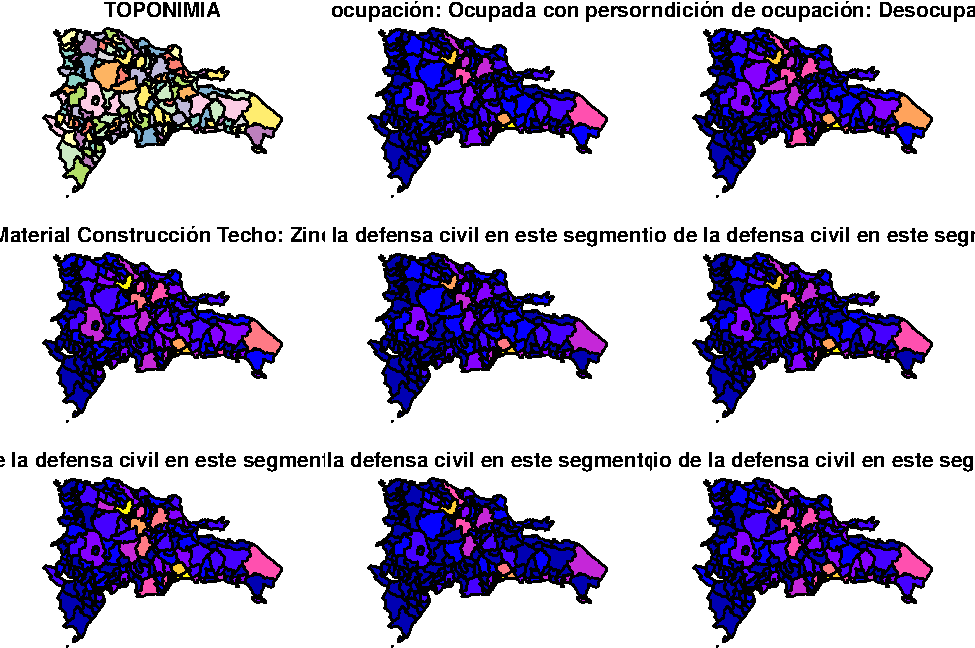
\includegraphics{proyecto_files/figure-latex/unnamed-chunk-2-1.pdf}

\begin{Shaded}
\begin{Highlighting}[]
\NormalTok{vivref }\OperatorTok\StringTok{ }\KeywordTok{mutate}\NormalTok{(}\DataTypeTok{vtotal=}
                    \StringTok{`}\DataTypeTok{Centros de refugio de la defensa civil en este segmento: Otros: Si}\StringTok{`}\OperatorTok{+}
\StringTok{                    `}\DataTypeTok{Centros de refugio de la defensa civil en este segmento: Centro deportivo: Si}\StringTok{`}\NormalTok{)}
\end{Highlighting}
\end{Shaded}

\begin{verbatim}
## Simple feature collection with 155 features and 20 fields
## geometry type:  MULTIPOLYGON
## dimension:      XY
## bbox:           xmin: -72.01147 ymin: 17.47033 xmax: -68.32354 ymax: 19.93211
## epsg (SRID):    4326
## proj4string:    +proj=longlat +datum=WGS84 +no_defs
## First 10 features:
##                  TOPONIMIA
## 1  SANTO DOMINGO DE GUZMÁN
## 2                     AZUA
## 3              LAS CHARCAS
## 4     LAS YAYAS DE VIAJAMA
## 5          PADRE LAS CASAS
## 6                  PERALTA
## 7             SABANA YEGUA
## 8             PUEBLO VIEJO
## 9            TÁBARA ARRIBA
## 10                GUAYABAL
##    Condición de ocupación: Ocupada con personas presentes
## 1                                                  288362
## 2                                                   22797
## 3                                                    3147
## 4                                                    4807
## 5                                                    5243
## 6                                                    3144
## 7                                                    4828
## 8                                                    2689
## 9                                                    4108
## 10                                                   1386
##    Condición de ocupación: Desocupada Material Construcción Techo: Zinc
## 1                               42200                             91950
## 2                                1920                             18544
## 3                                 944                              2919
## 4                                 798                              4475
## 5                                1345                              5874
## 6                                 446                              3019
## 7                                 594                              2549
## 8                                 208                              2294
## 9                                 426                              3737
## 10                                464                              1723
##    Centros de refugio de la defensa civil en este segmento: Escuela o Liceo: Si
## 1                                                                        174938
## 2                                                                         12706
## 3                                                                           763
## 4                                                                          3722
## 5                                                                          3400
## 6                                                                          2458
## 7                                                                          3206
## 8                                                                          2266
## 9                                                                          2239
## 10                                                                         1584
##    Centros de refugio de la defensa civil en este segmento: Iglesia: Si
## 1                                                                170337
## 2                                                                  9122
## 3                                                                   425
## 4                                                                  3421
## 5                                                                  1422
## 6                                                                   684
## 7                                                                   196
## 8                                                                    99
## 9                                                                   319
## 10                                                                  290
##    Centros de refugio de la defensa civil en este segmento: Salón comunal: Si
## 1                                                                       61706
## 2                                                                        4718
## 3                                                                           0
## 4                                                                         229
## 5                                                                         790
## 6                                                                         999
## 7                                                                          59
## 8                                                                         698
## 9                                                                         371
## 10                                                                          0
##    Centros de refugio de la defensa civil en este segmento: Centro deportivo: Si
## 1                                                                          77246
## 2                                                                           2525
## 3                                                                              0
## 4                                                                             52
## 5                                                                            434
## 6                                                                            262
## 7                                                                            969
## 8                                                                              0
## 9                                                                            178
## 10                                                                             0
##    Centros de refugio de la defensa civil en este segmento: Otros: Si
## 1                                                               71189
## 2                                                                4565
## 3                                                                   0
## 4                                                                 560
## 5                                                                1284
## 6                                                                1206
## 7                                                                2480
## 8                                                                   0
## 9                                                                 574
## 10                                                                679
##                              geom Total de viviendas
## 1  MULTIPOLYGON (((-69.89794 1...             330562
## 2  MULTIPOLYGON (((-70.71457 1...              24717
## 3  MULTIPOLYGON (((-70.50185 1...               4091
## 4  MULTIPOLYGON (((-70.85774 1...               5605
## 5  MULTIPOLYGON (((-70.77551 1...               6588
## 6  MULTIPOLYGON (((-70.73131 1...               3590
## 7  MULTIPOLYGON (((-70.83014 1...               5422
## 8  MULTIPOLYGON (((-70.79387 1...               2897
## 9  MULTIPOLYGON (((-70.83352 1...               4534
## 10 MULTIPOLYGON (((-70.68664 1...               1850
##    Condición de ocupación: Ocupada con personas presentes_PCT
## 1                                                       87.23
## 2                                                       92.23
## 3                                                       76.92
## 4                                                       85.76
## 5                                                       79.58
## 6                                                       87.58
## 7                                                       89.04
## 8                                                       92.82
## 9                                                       90.60
## 10                                                      74.92
##    Condición de ocupación: Desocupada_PCT
## 1                                   12.77
## 2                                    7.77
## 3                                   23.08
## 4                                   14.24
## 5                                   20.42
## 6                                   12.42
## 7                                   10.96
## 8                                    7.18
## 9                                    9.40
## 10                                  25.08
##    Material Construcción Techo: Zinc_PCT
## 1                                  27.82
## 2                                  75.03
## 3                                  71.35
## 4                                  79.84
## 5                                  89.16
## 6                                  84.09
## 7                                  47.01
## 8                                  79.19
## 9                                  82.42
## 10                                 93.14
##    Centros de refugio de la defensa civil en este segmento: Escuela o Liceo: Si_PCT
## 1                                                                             52.92
## 2                                                                             51.41
## 3                                                                             18.65
## 4                                                                             66.40
## 5                                                                             51.61
## 6                                                                             68.47
## 7                                                                             59.13
## 8                                                                             78.22
## 9                                                                             49.38
## 10                                                                            85.62
##    Centros de refugio de la defensa civil en este segmento: Iglesia: Si_PCT
## 1                                                                     51.53
## 2                                                                     36.91
## 3                                                                     10.39
## 4                                                                     61.03
## 5                                                                     21.58
## 6                                                                     19.05
## 7                                                                      3.61
## 8                                                                      3.42
## 9                                                                      7.04
## 10                                                                    15.68
##    Centros de refugio de la defensa civil en este segmento: Salón comunal: Si_PCT
## 1                                                                           18.67
## 2                                                                           19.09
## 3                                                                            0.00
## 4                                                                            4.09
## 5                                                                           11.99
## 6                                                                           27.83
## 7                                                                            1.09
## 8                                                                           24.09
## 9                                                                            8.18
## 10                                                                           0.00
##    Centros de refugio de la defensa civil en este segmento: Centro deportivo: Si_PCT
## 1                                                                              23.37
## 2                                                                              10.22
## 3                                                                               0.00
## 4                                                                               0.93
## 5                                                                               6.59
## 6                                                                               7.30
## 7                                                                              17.87
## 8                                                                               0.00
## 9                                                                               3.93
## 10                                                                              0.00
##    Centros de refugio de la defensa civil en este segmento: Otros: Si_PCT
## 1                                                                   21.54
## 2                                                                   18.47
## 3                                                                    0.00
## 4                                                                    9.99
## 5                                                                   19.49
## 6                                                                   33.59
## 7                                                                   45.74
## 8                                                                    0.00
## 9                                                                   12.66
## 10                                                                  36.70
##    Material Construcción Techo: Zinc_PCT log vtotal
## 1                                   3.325755 148435
## 2                                   4.317888   7090
## 3                                   4.267597      0
## 4                                   4.380025    612
## 5                                   4.490433   1718
## 6                                   4.431888   1468
## 7                                   3.850360   3449
## 8                                   4.371850      0
## 9                                   4.411828    752
## 10                                  4.534104    679
\end{verbatim}

\begin{Shaded}
\begin{Highlighting}[]
\NormalTok{vivref.sp <-}\StringTok{ }\KeywordTok{as_Spatial}\NormalTok{(vivref)}
\KeywordTok{colnames}\NormalTok{(vivref.sp}\OperatorTok{@}\NormalTok{data) <-}\StringTok{ }\NormalTok{vivref }\OperatorTok\StringTok{ }\KeywordTok{st_drop_geometry}\NormalTok{() }\OperatorTok\StringTok{ }\NormalTok{colnames}

\KeywordTok{row.names}\NormalTok{(vivref.sp) <-}\StringTok{ }\KeywordTok{as.character}\NormalTok{(vivref.sp}\OperatorTok{$}\NormalTok{TOPONIMIA)}

\CommentTok{#Utilizamos el criterio queen y de esta manera aplicamos la vecindad por contigüidad.}
\NormalTok{vivref.nb  <-}\StringTok{ }\KeywordTok{poly2nb}\NormalTok{(vivref.sp, }\DataTypeTok{queen=}\OtherTok{TRUE}\NormalTok{)}
\KeywordTok{summary}\NormalTok{(vivref.nb)}
\end{Highlighting}
\end{Shaded}

\begin{verbatim}
## Neighbour list object:
## Number of regions: 155 
## Number of nonzero links: 804 
## Percentage nonzero weights: 3.346514 
## Average number of links: 5.187097 
## Link number distribution:
## 
##  1  2  3  4  5  6  7  8  9 10 11 12 14 
##  1 10 20 34 33 22 13 13  4  1  1  2  1 
## 1 least connected region:
## JUAN DE HERRERA with 1 link
## 1 most connected region:
## LA VEGA with 14 links
\end{verbatim}

\begin{Shaded}
\begin{Highlighting}[]
\KeywordTok{card}\NormalTok{(vivref.nb)}
\end{Highlighting}
\end{Shaded}

\begin{verbatim}
##   [1]  4  6  3  6  7  6  3  2  6  5  5  7  5  8  4  3  4  7  4  3  5  6  4
##  [24]  4  4  8  5  5  4  6  4  5 12  4  5  6  7  4  5  3  3  4  4  6  5  8
##  [47]  3 10  3  7  3  2  3  3  5  7  8  5  2  4  5  3 14  8  7  3  6  2  5
##  [70]  4  5  4  8  5  2  3  5  2  6  3  8  7  4  5  6  4  5  4  2  7  4  4
##  [93]  2  7  2  9  3  3  5  6  5  2  6 11  4  8  1  7  5  4  6  5  5  5  4
## [116]  9  6  7  4 12  5  5  4  8  4  3  5  4  9  4  3  8  6  5  9  4  6  8
## [139]  7  6  8  4  6  6  4  8  3  6  5  4  6  4  5  5  5
\end{verbatim}

\begin{Shaded}
\begin{Highlighting}[]
\KeywordTok{sapply}\NormalTok{(vivref.nb, }\ControlFlowTok{function}\NormalTok{(x) x)}
\end{Highlighting}
\end{Shaded}

\begin{verbatim}
## [[1]]
## [1] 149 150 151 154
## 
## [[2]]
## [1]  6  7  8  9 11 27
## 
## [[3]]
## [1]  11  79 146
## 
## [[4]]
## [1]   5   6   9  14  21 104
## 
## [[5]]
## [1]   4   6  10  64  65 104 105
## 
## [[6]]
## [1]  2  4  5  9 10 11
## 
## [[7]]
## [1] 2 8 9
## 
## [[8]]
## [1] 2 7
## 
## [[9]]
## [1]  2  4  6  7 21 27
## 
## [[10]]
## [1]   5   6  11  64 146
## 
## [[11]]
## [1]   2   3   6  10 146
## 
## [[12]]
## [1]  13  14  15  56  57 106 109
## 
## [[13]]
## [1]  12  14  56  57 109
## 
## [[14]]
## [1]   4  12  13  21  22  56 104 109
## 
## [[15]]
## [1]  12  16  57 106
## 
## [[16]]
## [1]  15  55 106
## 
## [[17]]
## [1] 18 23 24 26
## 
## [[18]]
## [1] 17 22 23 24 25 26 56
## 
## [[19]]
## [1] 20 26 77 78
## 
## [[20]]
## [1] 19 23 26
## 
## [[21]]
## [1]  4  9 14 22 27
## 
## [[22]]
## [1] 14 18 21 24 27 56
## 
## [[23]]
## [1] 17 18 20 26
## 
## [[24]]
## [1] 17 18 22 27
## 
## [[25]]
## [1] 18 26 56 57
## 
## [[26]]
## [1] 17 18 19 20 23 25 57 77
## 
## [[27]]
## [1]  2  9 21 22 24
## 
## [[28]]
## [1] 29 30 71 74 75
## 
## [[29]]
## [1] 28 30 31 32
## 
## [[30]]
## [1]  28  29  32  73  74 129
## 
## [[31]]
## [1]  29  32  44 130
## 
## [[32]]
## [1]  29  30  31 129 130
## 
## [[33]]
##  [1]  35  36  38  50  63  67  69  70  90  91  92 118
## 
## [[34]]
## [1] 37 67 69 94
## 
## [[35]]
## [1] 33 36 37 39 69
## 
## [[36]]
## [1]  33  35  38  39 116 119
## 
## [[37]]
## [1]  34  35  39  69  94 117 140
## 
## [[38]]
## [1]  33  36 118 119
## 
## [[39]]
## [1]  35  36  37 116 117
## 
## [[40]]
## [1]  41  42 108
## 
## [[41]]
## [1]  40  44 108
## 
## [[42]]
## [1]  40  43  45 108
## 
## [[43]]
## [1] 42 45 54 55
## 
## [[44]]
## [1]  31  41 104 108 129 130
## 
## [[45]]
## [1]  42  43  55 106 108
## 
## [[46]]
## [1]  47  58  61 112 113 143 144 145
## 
## [[47]]
## [1]  46  58 144
## 
## [[48]]
##  [1]  49  50  51  63  81  87  90 123 125 127
## 
## [[49]]
## [1] 48 63 90
## 
## [[50]]
## [1] 33 48 51 70 87 90 91
## 
## [[51]]
## [1] 48 50 87
## 
## [[52]]
## [1] 53 54
## 
## [[53]]
## [1] 52 57 77
## 
## [[54]]
## [1] 43 52 55
## 
## [[55]]
## [1]  16  43  45  54 106
## 
## [[56]]
## [1] 12 13 14 18 22 25 57
## 
## [[57]]
## [1] 12 13 15 25 26 53 56 77
## 
## [[58]]
## [1] 46 47 59 60 61
## 
## [[59]]
## [1] 58 60
## 
## [[60]]
## [1] 58 59 61 62
## 
## [[61]]
## [1]  46  58  60  62 112
## 
## [[62]]
## [1]  60  61 112
## 
## [[63]]
##  [1]  33  48  49  64  65  66  90  92 118 120 122 127 128 135
## 
## [[64]]
## [1]   5  10  63  65 135 146 147 148
## 
## [[65]]
## [1]   5  63  64 105 122 124 135
## 
## [[66]]
## [1]  63 118 135
## 
## [[67]]
## [1] 33 34 68 69 70 94
## 
## [[68]]
## [1] 67 70
## 
## [[69]]
## [1] 33 34 35 37 67
## 
## [[70]]
## [1] 33 50 67 68
## 
## [[71]]
## [1] 28 72 74 75 76
## 
## [[72]]
## [1] 71 73 74 76
## 
## [[73]]
## [1]  30  72  74  76  88 129 132 134
## 
## [[74]]
## [1] 28 30 71 72 73
## 
## [[75]]
## [1] 28 71
## 
## [[76]]
## [1] 71 72 73
## 
## [[77]]
## [1] 19 26 53 57 78
## 
## [[78]]
## [1] 19 77
## 
## [[79]]
## [1]   3  80  99 101 103 146
## 
## [[80]]
## [1]  79  97 101
## 
## [[81]]
## [1]  48  82  84  86  87  89 120 125
## 
## [[82]]
## [1]  81  83  84 120 121 126 133
## 
## [[83]]
## [1]  82  84  85 133
## 
## [[84]]
## [1] 81 82 83 85 86
## 
## [[85]]
## [1]  83  84  86  88 133 134
## 
## [[86]]
## [1] 81 84 85 88
## 
## [[87]]
## [1] 48 50 51 81 89
## 
## [[88]]
## [1]  73  85  86 134
## 
## [[89]]
## [1] 81 87
## 
## [[90]]
## [1] 33 48 49 50 63 91 92
## 
## [[91]]
## [1] 33 50 90 92
## 
## [[92]]
## [1] 33 63 90 91
## 
## [[93]]
## [1] 94 95
## 
## [[94]]
## [1]  34  37  67  93  95 140 144
## 
## [[95]]
## [1] 93 94
## 
## [[96]]
## [1]  97  98  99 100 101 102 150 154 155
## 
## [[97]]
## [1]  80  96 101
## 
## [[98]]
## [1]  96 102 150
## 
## [[99]]
## [1]  79  96 100 101 103
## 
## [[100]]
## [1]  96  99 103 137 141 155
## 
## [[101]]
## [1] 79 80 96 97 99
## 
## [[102]]
## [1] 96 98
## 
## [[103]]
## [1]  79  99 100 137 146 148
## 
## [[104]]
##  [1]   4   5  14  44 105 106 107 108 109 124 129
## 
## [[105]]
## [1]   5  65 104 124
## 
## [[106]]
## [1]  12  15  16  45  55 104 108 109
## 
## [[107]]
## [1] 104
## 
## [[108]]
## [1]  40  41  42  44  45 104 106
## 
## [[109]]
## [1]  12  13  14 104 106
## 
## [[110]]
## [1] 112 113 114 115
## 
## [[111]]
## [1] 114 115 139 143 152 153
## 
## [[112]]
## [1]  46  61  62 110 113
## 
## [[113]]
## [1]  46 110 112 114 143
## 
## [[114]]
## [1] 110 111 113 115 143
## 
## [[115]]
## [1] 110 111 114 152
## 
## [[116]]
## [1]  36  39 117 118 119 135 136 141 142
## 
## [[117]]
## [1]  37  39 116 138 140 142
## 
## [[118]]
## [1]  33  38  63  66 116 119 135
## 
## [[119]]
## [1]  36  38 116 118
## 
## [[120]]
##  [1]  63  81  82 121 122 123 124 125 126 127 128 132
## 
## [[121]]
## [1]  82 120 126 132 133
## 
## [[122]]
## [1]  63  65 120 124 128
## 
## [[123]]
## [1]  48 120 125 127
## 
## [[124]]
## [1]  65 104 105 120 122 129 131 132
## 
## [[125]]
## [1]  48  81 120 123
## 
## [[126]]
## [1]  82 120 121
## 
## [[127]]
## [1]  48  63 120 123 128
## 
## [[128]]
## [1]  63 120 122 127
## 
## [[129]]
## [1]  30  32  44  73 104 124 130 131 132
## 
## [[130]]
## [1]  31  32  44 129
## 
## [[131]]
## [1] 124 129 132
## 
## [[132]]
## [1]  73 120 121 124 129 131 133 134
## 
## [[133]]
## [1]  82  83  85 121 132 134
## 
## [[134]]
## [1]  73  85  88 132 133
## 
## [[135]]
## [1]  63  64  65  66 116 118 136 137 148
## 
## [[136]]
## [1] 116 135 137 141
## 
## [[137]]
## [1] 100 103 135 136 141 148
## 
## [[138]]
## [1] 117 139 140 141 142 149 151 153
## 
## [[139]]
## [1] 111 138 140 143 144 145 153
## 
## [[140]]
## [1]  37  94 117 138 139 144
## 
## [[141]]
## [1] 100 116 136 137 138 142 151 155
## 
## [[142]]
## [1] 116 117 138 141
## 
## [[143]]
## [1]  46 111 113 114 139 145
## 
## [[144]]
## [1]  46  47  94 139 140 145
## 
## [[145]]
## [1]  46 139 143 144
## 
## [[146]]
## [1]   3  10  11  64  79 103 147 148
## 
## [[147]]
## [1]  64 146 148
## 
## [[148]]
## [1]  64 103 135 137 146 147
## 
## [[149]]
## [1]   1 138 151 152 153
## 
## [[150]]
## [1]   1  96  98 154
## 
## [[151]]
## [1]   1 138 141 149 154 155
## 
## [[152]]
## [1] 111 115 149 153
## 
## [[153]]
## [1] 111 138 139 149 152
## 
## [[154]]
## [1]   1  96 150 151 155
## 
## [[155]]
## [1]  96 100 141 151 154
\end{verbatim}

\begin{Shaded}
\begin{Highlighting}[]
\CommentTok{#Realizamos un mapa de los vínculos de vecindad y confirmamos si el objeto de vencidad es simétrico.}
\KeywordTok{plot}\NormalTok{(vivref.sp, }\DataTypeTok{border=}\StringTok{"grey"}\NormalTok{, }\DataTypeTok{lwd=}\FloatTok{0.5}\NormalTok{)}
\KeywordTok{plot}\NormalTok{(vivref.nb, }\KeywordTok{coordinates}\NormalTok{(vivref.sp), }\DataTypeTok{add=}\NormalTok{T)}
\end{Highlighting}
\end{Shaded}

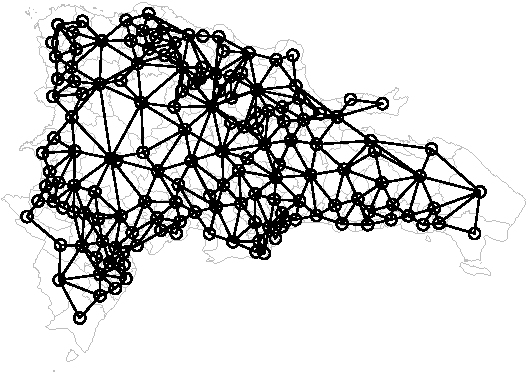
\includegraphics{proyecto_files/figure-latex/unnamed-chunk-2-2.pdf}

\begin{Shaded}
\begin{Highlighting}[]
\KeywordTok{is.symmetric.nb}\NormalTok{(vivref.nb)}
\end{Highlighting}
\end{Shaded}

\begin{verbatim}
## [1] TRUE
\end{verbatim}

\begin{Shaded}
\begin{Highlighting}[]
\NormalTok{coords <-}\StringTok{ }\KeywordTok{coordinates}\NormalTok{(vivref.sp)}
\NormalTok{ident <-}\StringTok{ }\KeywordTok{row.names}\NormalTok{(vivref.sp)}
\NormalTok{vivref.nb.k1  <-}\StringTok{ }\KeywordTok{knn2nb}\NormalTok{(}\KeywordTok{knearneigh}\NormalTok{(coords, }\DataTypeTok{k =} \DecValTok{1}\NormalTok{), }\DataTypeTok{row.names =}\NormalTok{ ident)}
\KeywordTok{summary}\NormalTok{(vivref.nb.k1)}
\end{Highlighting}
\end{Shaded}

\begin{verbatim}
## Neighbour list object:
## Number of regions: 155 
## Number of nonzero links: 155 
## Percentage nonzero weights: 0.6451613 
## Average number of links: 1 
## Non-symmetric neighbours list
## Link number distribution:
## 
##   1 
## 155 
## 155 least connected regions:
## SANTO DOMINGO DE GUZMÁN AZUA LAS CHARCAS LAS YAYAS DE VIAJAMA PADRE LAS CASAS PERALTA SABANA YEGUA PUEBLO VIEJO TÁBARA ARRIBA GUAYABAL ESTEBANÍA NEIBA GALVÁN TAMAYO VILLA JARAGUA LOS RÍOS BARAHONA CABRAL ENRIQUILLO PARAÍSO VICENTE NOBLE EL PEÑÓN LA CIÉNAGA FUNDACIÓN LAS SALINAS POLO JAQUIMEYES DAJABÓN LOMA DE CABRERA PARTIDO RESTAURACIÓN EL PINO SAN FRANCISCO DE MACORÍS ARENOSO CASTILLO PIMENTEL VILLA RIVA LAS GUÁRANAS EUGENIO MARÍA DE HOSTOS COMENDADOR BÁNICA EL LLANO HONDO VALLE PEDRO SANTANA JUAN SANTIAGO EL SEIBO MICHES MOCA CAYETANO GERMOSÉN GASPAR HERNÁNDEZ JAMAO AL NORTE JIMANÍ DUVERGÉ LA DESCUBIERTA POSTRER RÍO CRISTÓBAL MELLA HIGÜEY SAN RAFAEL DEL YUMA LA ROMANA GUAYMATE VILLA HERMOSA LA VEGA CONSTANZA JARABACOA JIMA ABAJO NAGUA CABRERA EL FACTOR RÍO SAN JUAN MONTE CRISTI CASTAÑUELAS GUAYUBÍN LAS MATAS DE SANTA CRUZ PEPILLO SALCEDO VILLA VÁSQUEZ PEDERNALES OVIEDO BANÍ NIZAO PUERTO PLATA ALTAMIRA GUANANICO IMBERT LOS HIDALGOS LUPERÓN SOSÚA VILLA ISABELA VILLA MONTELLANO SALCEDO TENARES VILLA TAPIA SAMANÁ SÁNCHEZ LAS TERRENAS SAN CRISTÓBAL SABANA GRANDE DE PALENQUE BAJOS DE HAINA CAMBITA GARABITOS VILLA ALTAGRACIA YAGUATE SAN GREGORIO DE NIGUA LOS CACAOS SAN JUAN BOHECHÍO EL CERCADO JUAN DE HERRERA LAS MATAS DE FARFÁN VALLEJUELO SAN PEDRO DE MACORÍS LOS LLANOS RAMÓN SANTANA CONSUELO QUISQUEYA GUAYACANES COTUÍ CEVICOS FANTINO LA MATA SANTIAGO BISONÓ JÁNICO LICEY AL MEDIO SAN JOSÉ DE LAS MATAS TAMBORIL VILLA GONZÁLEZ PUÑAL SABANA IGLESIA SAN IGNACIO DE SABANETA VILLA LOS ALMÁCIGOS MONCIÓN MAO ESPERANZA LAGUNA SALADA BONAO MAIMÓN PIEDRA BLANCA MONTE PLATA BAYAGUANA SABANA GRANDE DE BOYÁ YAMASÁ PERALVILLO HATO MAYOR SABANA DE LA MAR EL VALLE SAN JOSÉ DE OCOA SABANA LARGA RANCHO ARRIBA SANTO DOMINGO ESTE SANTO DOMINGO OESTE SANTO DOMINGO NORTE BOCA CHICA SAN ANTONIO DE GUERRA LOS ALCARRIZOS PEDRO BRAND with 1 link
## 155 most connected regions:
## SANTO DOMINGO DE GUZMÁN AZUA LAS CHARCAS LAS YAYAS DE VIAJAMA PADRE LAS CASAS PERALTA SABANA YEGUA PUEBLO VIEJO TÁBARA ARRIBA GUAYABAL ESTEBANÍA NEIBA GALVÁN TAMAYO VILLA JARAGUA LOS RÍOS BARAHONA CABRAL ENRIQUILLO PARAÍSO VICENTE NOBLE EL PEÑÓN LA CIÉNAGA FUNDACIÓN LAS SALINAS POLO JAQUIMEYES DAJABÓN LOMA DE CABRERA PARTIDO RESTAURACIÓN EL PINO SAN FRANCISCO DE MACORÍS ARENOSO CASTILLO PIMENTEL VILLA RIVA LAS GUÁRANAS EUGENIO MARÍA DE HOSTOS COMENDADOR BÁNICA EL LLANO HONDO VALLE PEDRO SANTANA JUAN SANTIAGO EL SEIBO MICHES MOCA CAYETANO GERMOSÉN GASPAR HERNÁNDEZ JAMAO AL NORTE JIMANÍ DUVERGÉ LA DESCUBIERTA POSTRER RÍO CRISTÓBAL MELLA HIGÜEY SAN RAFAEL DEL YUMA LA ROMANA GUAYMATE VILLA HERMOSA LA VEGA CONSTANZA JARABACOA JIMA ABAJO NAGUA CABRERA EL FACTOR RÍO SAN JUAN MONTE CRISTI CASTAÑUELAS GUAYUBÍN LAS MATAS DE SANTA CRUZ PEPILLO SALCEDO VILLA VÁSQUEZ PEDERNALES OVIEDO BANÍ NIZAO PUERTO PLATA ALTAMIRA GUANANICO IMBERT LOS HIDALGOS LUPERÓN SOSÚA VILLA ISABELA VILLA MONTELLANO SALCEDO TENARES VILLA TAPIA SAMANÁ SÁNCHEZ LAS TERRENAS SAN CRISTÓBAL SABANA GRANDE DE PALENQUE BAJOS DE HAINA CAMBITA GARABITOS VILLA ALTAGRACIA YAGUATE SAN GREGORIO DE NIGUA LOS CACAOS SAN JUAN BOHECHÍO EL CERCADO JUAN DE HERRERA LAS MATAS DE FARFÁN VALLEJUELO SAN PEDRO DE MACORÍS LOS LLANOS RAMÓN SANTANA CONSUELO QUISQUEYA GUAYACANES COTUÍ CEVICOS FANTINO LA MATA SANTIAGO BISONÓ JÁNICO LICEY AL MEDIO SAN JOSÉ DE LAS MATAS TAMBORIL VILLA GONZÁLEZ PUÑAL SABANA IGLESIA SAN IGNACIO DE SABANETA VILLA LOS ALMÁCIGOS MONCIÓN MAO ESPERANZA LAGUNA SALADA BONAO MAIMÓN PIEDRA BLANCA MONTE PLATA BAYAGUANA SABANA GRANDE DE BOYÁ YAMASÁ PERALVILLO HATO MAYOR SABANA DE LA MAR EL VALLE SAN JOSÉ DE OCOA SABANA LARGA RANCHO ARRIBA SANTO DOMINGO ESTE SANTO DOMINGO OESTE SANTO DOMINGO NORTE BOCA CHICA SAN ANTONIO DE GUERRA LOS ALCARRIZOS PEDRO BRAND with 1 link
\end{verbatim}

\begin{Shaded}
\begin{Highlighting}[]
\KeywordTok{card}\NormalTok{(vivref.nb.k1)}
\end{Highlighting}
\end{Shaded}

\begin{verbatim}
##   [1] 1 1 1 1 1 1 1 1 1 1 1 1 1 1 1 1 1 1 1 1 1 1 1 1 1 1 1 1 1 1 1 1 1 1 1
##  [36] 1 1 1 1 1 1 1 1 1 1 1 1 1 1 1 1 1 1 1 1 1 1 1 1 1 1 1 1 1 1 1 1 1 1 1
##  [71] 1 1 1 1 1 1 1 1 1 1 1 1 1 1 1 1 1 1 1 1 1 1 1 1 1 1 1 1 1 1 1 1 1 1 1
## [106] 1 1 1 1 1 1 1 1 1 1 1 1 1 1 1 1 1 1 1 1 1 1 1 1 1 1 1 1 1 1 1 1 1 1 1
## [141] 1 1 1 1 1 1 1 1 1 1 1 1 1 1 1
\end{verbatim}

\begin{Shaded}
\begin{Highlighting}[]
\KeywordTok{sapply}\NormalTok{(vivref.nb.k1, }\ControlFlowTok{function}\NormalTok{(x) x)}
\end{Highlighting}
\end{Shaded}

\begin{verbatim}
##   [1] 150   8  79   9 105  10   9   2   7   6   2  15  12  21  12  15  24
##  [18]  17  20  23  27  24  17  22  18  18  21  75  32  32  29  30  38  37
##  [35]  39  38  34  36  35  41  40  45  45 130  43  47  46 125  92  91  87
##  [52]  54  57  55  16  22  25  59  60  61  60  60  49  10 122 118  69  70
##  [69]  67  68  72  76  76  72  28  72  53  19   3  97  89 126  84  83  83
##  [86]  85  51  85  81  91  90  49  95  34  94 102  80 150  96 103  80  96
## [103] 100 107   5  45 104  41 106 113 114  62 110 115 114 119  39 119 118
## [120] 126 126 128 127 131 123 121 123 127 130  32 129 133  83  85 137 137
## [137] 136 151 111 117 142 141 113 145 144 147 146 147 153  98   1 153 152
## [154] 150 154
\end{verbatim}

\begin{Shaded}
\begin{Highlighting}[]
\KeywordTok{plot}\NormalTok{(vivref.sp, }\DataTypeTok{border=}\StringTok{"grey"}\NormalTok{, }\DataTypeTok{lwd=}\FloatTok{0.5}\NormalTok{)}
\KeywordTok{plot}\NormalTok{(vivref.nb.k1, }\KeywordTok{coordinates}\NormalTok{(vivref.sp), }\DataTypeTok{add=}\NormalTok{T)}
\end{Highlighting}
\end{Shaded}

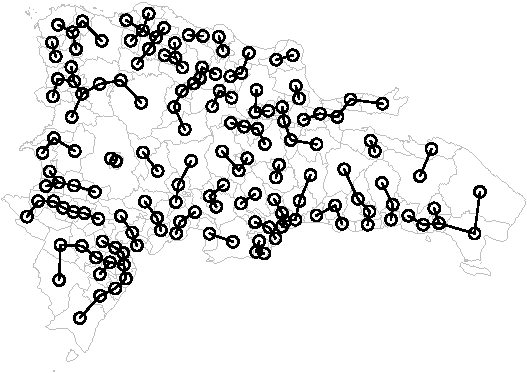
\includegraphics{proyecto_files/figure-latex/unnamed-chunk-2-3.pdf}

\begin{Shaded}
\begin{Highlighting}[]
\KeywordTok{is.symmetric.nb}\NormalTok{(vivref.nb.k1)}
\end{Highlighting}
\end{Shaded}

\begin{verbatim}
## [1] FALSE
\end{verbatim}

\begin{Shaded}
\begin{Highlighting}[]
\NormalTok{dist<-}\StringTok{ }\KeywordTok{unlist}\NormalTok{(}\KeywordTok{nbdists}\NormalTok{(vivref.nb.k1, coords))}
\KeywordTok{summary}\NormalTok{(dist)}
\end{Highlighting}
\end{Shaded}

\begin{verbatim}
##    Min. 1st Qu.  Median    Mean 3rd Qu.    Max. 
## 0.04036 0.08754 0.10140 0.11396 0.12765 0.28058
\end{verbatim}

\begin{Shaded}
\begin{Highlighting}[]
\KeywordTok{hist}\NormalTok{(dist)}
\end{Highlighting}
\end{Shaded}

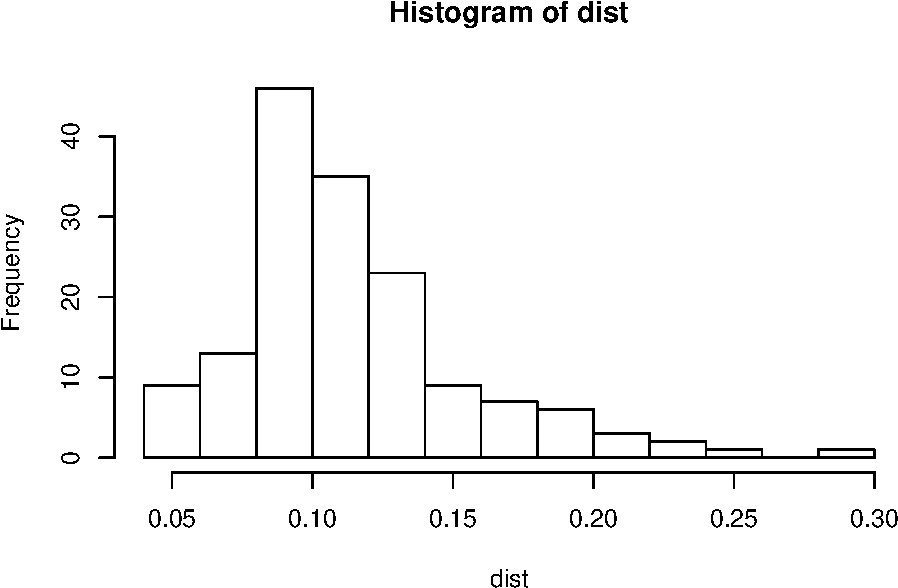
\includegraphics{proyecto_files/figure-latex/unnamed-chunk-2-4.pdf}

\begin{Shaded}
\begin{Highlighting}[]
\KeywordTok{boxplot}\NormalTok{(dist)}
\end{Highlighting}
\end{Shaded}

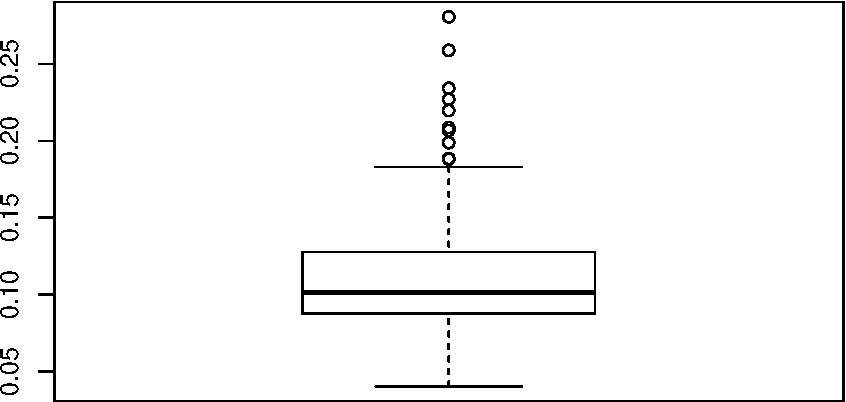
\includegraphics{proyecto_files/figure-latex/unnamed-chunk-2-5.pdf}

\begin{Shaded}
\begin{Highlighting}[]
\NormalTok{(distmin <-}\StringTok{ }\KeywordTok{min}\NormalTok{(dist)) }
\end{Highlighting}
\end{Shaded}

\begin{verbatim}
## [1] 0.04036477
\end{verbatim}

\begin{Shaded}
\begin{Highlighting}[]
\NormalTok{(distmax <-}\StringTok{ }\KeywordTok{max}\NormalTok{(dist))}
\end{Highlighting}
\end{Shaded}

\begin{verbatim}
## [1] 0.2805772
\end{verbatim}

\begin{Shaded}
\begin{Highlighting}[]
\NormalTok{indicemin <-}\StringTok{ }\KeywordTok{which}\NormalTok{(dist}\OperatorTok{==}\NormalTok{distmin)}
\NormalTok{ident[indicemin]}
\end{Highlighting}
\end{Shaded}

\begin{verbatim}
## [1] "SAN JUAN"        "JUAN DE HERRERA"
\end{verbatim}

\begin{Shaded}
\begin{Highlighting}[]
\NormalTok{indicemax <-}\StringTok{ }\KeywordTok{which}\NormalTok{(dist}\OperatorTok{==}\NormalTok{distmax)}
\NormalTok{ident[indicemax]}
\end{Highlighting}
\end{Shaded}

\begin{verbatim}
## [1] "HIGÜEY"
\end{verbatim}

\begin{Shaded}
\begin{Highlighting}[]
\NormalTok{ident[}\KeywordTok{order}\NormalTok{(dist)]}
\end{Highlighting}
\end{Shaded}

\begin{verbatim}
##   [1] "SAN JUAN"                  "JUAN DE HERRERA"          
##   [3] "BAJOS DE HAINA"            "SANTO DOMINGO OESTE"      
##   [5] "LICEY AL MEDIO"            "PUÑAL"                    
##   [7] "NIZAO"                     "SABANA GRANDE DE PALENQUE"
##   [9] "LOS ALCARRIZOS"            "EL PEÑÓN"                 
##  [11] "FUNDACIÓN"                 "SANTO DOMINGO DE GUZMÁN"  
##  [13] "TAMBORIL"                  "YAGUATE"                  
##  [15] "SABANA DE LA MAR"          "EL VALLE"                 
##  [17] "NEIBA"                     "VILLA JARAGUA"            
##  [19] "BISONÓ"                    "VILLA GONZÁLEZ"           
##  [21] "LOS RÍOS"                  "BARAHONA"                 
##  [23] "POSTRER RÍO"               "SALCEDO"                  
##  [25] "TENARES"                   "SANTIAGO"                 
##  [27] "AZUA"                      "PUEBLO VIEJO"             
##  [29] "GUANANICO"                 "IMBERT"                   
##  [31] "SAN JOSÉ DE OCOA"          "SABANA LARGA"             
##  [33] "SAN CRISTÓBAL"             "SAN GREGORIO DE NIGUA"    
##  [35] "SABANA YEGUA"              "TÁBARA ARRIBA"            
##  [37] "NAGUA"                     "EL FACTOR"                
##  [39] "YAMASÁ"                    "PERALVILLO"               
##  [41] "QUISQUEYA"                 "GUAYACANES"               
##  [43] "ESPERANZA"                 "VICENTE NOBLE"            
##  [45] "JAQUIMEYES"                "LA CIÉNAGA"               
##  [47] "PIMENTEL"                  "LAS GUÁRANAS"             
##  [49] "HONDO VALLE"               "JUAN SANTIAGO"            
##  [51] "FANTINO"                   "LA MATA"                  
##  [53] "CASTILLO"                  "EUGENIO MARÍA DE HOSTOS"  
##  [55] "JIMA ABAJO"                "CAYETANO GERMOSÉN"        
##  [57] "VILLA TAPIA"               "ALTAMIRA"                 
##  [59] "EL LLANO"                  "DAJABÓN"                  
##  [61] "PEPILLO SALCEDO"           "PARTIDO"                  
##  [63] "EL PINO"                   "SABANA IGLESIA"           
##  [65] "CRISTÓBAL"                 "JAMAO AL NORTE"           
##  [67] "SOSÚA"                     "PARAÍSO"                  
##  [69] "VILLA LOS ALMÁCIGOS"       "CABRAL"                   
##  [71] "SAN PEDRO DE MACORÍS"      "CONSUELO"                 
##  [73] "PUERTO PLATA"              "VILLA MONTELLANO"         
##  [75] "CASTAÑUELAS"               "VILLA VÁSQUEZ"            
##  [77] "MAIMÓN"                    "PIEDRA BLANCA"            
##  [79] "LAS SALINAS"               "MOCA"                     
##  [81] "LA ROMANA"                 "GUAYMATE"                 
##  [83] "LOS HIDALGOS"              "GALVÁN"                   
##  [85] "CAMBITA GARABITOS"         "POLO"                     
##  [87] "PEDRO BRAND"               "LA DESCUBIERTA"           
##  [89] "LAGUNA SALADA"             "EL CERCADO"               
##  [91] "VILLA HERMOSA"             "MONTE CRISTI"             
##  [93] "COTUÍ"                     "LAS MATAS DE SANTA CRUZ"  
##  [95] "LA VEGA"                   "LOMA DE CABRERA"          
##  [97] "PERALTA"                   "GUAYABAL"                 
##  [99] "LOS LLANOS"                "ENRIQUILLO"               
## [101] "VILLA ALTAGRACIA"          "LOS CACAOS"               
## [103] "LUPERÓN"                   "RAMÓN SANTANA"            
## [105] "JÁNICO"                    "CABRERA"                  
## [107] "RÍO SAN JUAN"              "RESTAURACIÓN"             
## [109] "RANCHO ARRIBA"             "ESTEBANÍA"                
## [111] "ARENOSO"                   "VILLA RIVA"               
## [113] "SÁNCHEZ"                   "MELLA"                    
## [115] "COMENDADOR"                "BÁNICA"                   
## [117] "SANTO DOMINGO NORTE"       "MAO"                      
## [119] "JIMANÍ"                    "BOCA CHICA"               
## [121] "SAN ANTONIO DE GUERRA"     "CEVICOS"                  
## [123] "VILLA ISABELA"             "TAMAYO"                   
## [125] "LAS YAYAS DE VIAJAMA"      "SAN IGNACIO DE SABANETA"  
## [127] "GASPAR HERNÁNDEZ"          "SANTO DOMINGO ESTE"       
## [129] "LAS TERRENAS"              "SAN FRANCISCO DE MACORÍS" 
## [131] "DUVERGÉ"                   "MONCIÓN"                  
## [133] "VALLEJUELO"                "PADRE LAS CASAS"          
## [135] "BOHECHÍO"                  "HATO MAYOR"               
## [137] "JARABACOA"                 "LAS MATAS DE FARFÁN"      
## [139] "PEDRO SANTANA"             "BONAO"                    
## [141] "LAS CHARCAS"               "BANÍ"                     
## [143] "SABANA GRANDE DE BOYÁ"     "CONSTANZA"                
## [145] "GUAYUBÍN"                  "MONTE PLATA"              
## [147] "EL SEIBO"                  "MICHES"                   
## [149] "OVIEDO"                    "SAN JOSÉ DE LAS MATAS"    
## [151] "BAYAGUANA"                 "SAMANÁ"                   
## [153] "PEDERNALES"                "SAN RAFAEL DEL YUMA"      
## [155] "HIGÜEY"
\end{verbatim}

\begin{Shaded}
\begin{Highlighting}[]
\NormalTok{vivref.w.W  <-}\StringTok{ }\KeywordTok{nb2listw}\NormalTok{(vivref.nb)}
\NormalTok{vivref.w.W}
\end{Highlighting}
\end{Shaded}

\begin{verbatim}
## Characteristics of weights list object:
## Neighbour list object:
## Number of regions: 155 
## Number of nonzero links: 804 
## Percentage nonzero weights: 3.346514 
## Average number of links: 5.187097 
## 
## Weights style: W 
## Weights constants summary:
##     n    nn  S0       S1       S2
## W 155 24025 155 65.94606 650.7687
\end{verbatim}

\begin{Shaded}
\begin{Highlighting}[]
\NormalTok{vivref.w.B <-}\StringTok{ }\KeywordTok{nb2listw}\NormalTok{(vivref.nb, }\DataTypeTok{style =} \StringTok{'B'}\NormalTok{)}
\NormalTok{vivref.w.B }
\end{Highlighting}
\end{Shaded}

\begin{verbatim}
## Characteristics of weights list object:
## Neighbour list object:
## Number of regions: 155 
## Number of nonzero links: 804 
## Percentage nonzero weights: 3.346514 
## Average number of links: 5.187097 
## 
## Weights style: B 
## Weights constants summary:
##     n    nn  S0   S1    S2
## B 155 24025 804 1608 19520
\end{verbatim}

\begin{Shaded}
\begin{Highlighting}[]
\KeywordTok{st_crs}\NormalTok{(vivref)}
\end{Highlighting}
\end{Shaded}

\begin{verbatim}
## Coordinate Reference System:
##   EPSG: 4326 
##   proj4string: "+proj=longlat +datum=WGS84 +no_defs"
\end{verbatim}

\begin{Shaded}
\begin{Highlighting}[]
\NormalTok{crsdestino <-}\StringTok{ }\DecValTok{32619}
\NormalTok{vivrefutm <-}\StringTok{ }\NormalTok{vivref }\OperatorTok\StringTok{ }\KeywordTok{st_transform}\NormalTok{(}\DataTypeTok{crs =}\NormalTok{ crsdestino)}

\CommentTok{#Variable en su versión original como transformada}
\NormalTok{coordsxy <-}\StringTok{ }\NormalTok{vivref }\OperatorTok
\StringTok{  }\KeywordTok{st_centroid}\NormalTok{() }\OperatorTok\StringTok{ }
\StringTok{  }\KeywordTok{mutate}\NormalTok{(}\DataTypeTok{x=}\KeywordTok{unlist}\NormalTok{(}\KeywordTok{map}\NormalTok{(geom,}\DecValTok{1}\NormalTok{)),}
         \DataTypeTok{y=}\KeywordTok{unlist}\NormalTok{(}\KeywordTok{map}\NormalTok{(geom,}\DecValTok{2}\NormalTok{))) }\OperatorTok
\StringTok{  }\KeywordTok{select}\NormalTok{(TOPONIMIA, x, y) }\OperatorTok\StringTok{ }
\StringTok{  }\KeywordTok{st_drop_geometry}\NormalTok{()}
\end{Highlighting}
\end{Shaded}

\begin{verbatim}
## Warning in st_centroid.sf(.): st_centroid assumes attributes are constant
## over geometries of x
\end{verbatim}

\begin{verbatim}
## Warning in st_centroid.sfc(st_geometry(x), of_largest_polygon =
## of_largest_polygon): st_centroid does not give correct centroids for
## longitude/latitude data
\end{verbatim}

\begin{Shaded}
\begin{Highlighting}[]
\NormalTok{vivrefconxy <-}\StringTok{ }\NormalTok{vivref }\OperatorTok
\StringTok{  }\KeywordTok{inner_join}\NormalTok{(coordsxy, }\DataTypeTok{by =} \StringTok{'TOPONIMIA'}\NormalTok{)}
\NormalTok{vivrefconxy}
\end{Highlighting}
\end{Shaded}

\begin{verbatim}
## Simple feature collection with 155 features and 21 fields
## geometry type:  MULTIPOLYGON
## dimension:      XY
## bbox:           xmin: -72.01147 ymin: 17.47033 xmax: -68.32354 ymax: 19.93211
## epsg (SRID):    4326
## proj4string:    +proj=longlat +datum=WGS84 +no_defs
## First 10 features:
##                  TOPONIMIA
## 1  SANTO DOMINGO DE GUZMÁN
## 2                     AZUA
## 3              LAS CHARCAS
## 4     LAS YAYAS DE VIAJAMA
## 5          PADRE LAS CASAS
## 6                  PERALTA
## 7             SABANA YEGUA
## 8             PUEBLO VIEJO
## 9            TÁBARA ARRIBA
## 10                GUAYABAL
##    Condición de ocupación: Ocupada con personas presentes
## 1                                                  288362
## 2                                                   22797
## 3                                                    3147
## 4                                                    4807
## 5                                                    5243
## 6                                                    3144
## 7                                                    4828
## 8                                                    2689
## 9                                                    4108
## 10                                                   1386
##    Condición de ocupación: Desocupada Material Construcción Techo: Zinc
## 1                               42200                             91950
## 2                                1920                             18544
## 3                                 944                              2919
## 4                                 798                              4475
## 5                                1345                              5874
## 6                                 446                              3019
## 7                                 594                              2549
## 8                                 208                              2294
## 9                                 426                              3737
## 10                                464                              1723
##    Centros de refugio de la defensa civil en este segmento: Escuela o Liceo: Si
## 1                                                                        174938
## 2                                                                         12706
## 3                                                                           763
## 4                                                                          3722
## 5                                                                          3400
## 6                                                                          2458
## 7                                                                          3206
## 8                                                                          2266
## 9                                                                          2239
## 10                                                                         1584
##    Centros de refugio de la defensa civil en este segmento: Iglesia: Si
## 1                                                                170337
## 2                                                                  9122
## 3                                                                   425
## 4                                                                  3421
## 5                                                                  1422
## 6                                                                   684
## 7                                                                   196
## 8                                                                    99
## 9                                                                   319
## 10                                                                  290
##    Centros de refugio de la defensa civil en este segmento: Salón comunal: Si
## 1                                                                       61706
## 2                                                                        4718
## 3                                                                           0
## 4                                                                         229
## 5                                                                         790
## 6                                                                         999
## 7                                                                          59
## 8                                                                         698
## 9                                                                         371
## 10                                                                          0
##    Centros de refugio de la defensa civil en este segmento: Centro deportivo: Si
## 1                                                                          77246
## 2                                                                           2525
## 3                                                                              0
## 4                                                                             52
## 5                                                                            434
## 6                                                                            262
## 7                                                                            969
## 8                                                                              0
## 9                                                                            178
## 10                                                                             0
##    Centros de refugio de la defensa civil en este segmento: Otros: Si
## 1                                                               71189
## 2                                                                4565
## 3                                                                   0
## 4                                                                 560
## 5                                                                1284
## 6                                                                1206
## 7                                                                2480
## 8                                                                   0
## 9                                                                 574
## 10                                                                679
##    Total de viviendas
## 1              330562
## 2               24717
## 3                4091
## 4                5605
## 5                6588
## 6                3590
## 7                5422
## 8                2897
## 9                4534
## 10               1850
##    Condición de ocupación: Ocupada con personas presentes_PCT
## 1                                                       87.23
## 2                                                       92.23
## 3                                                       76.92
## 4                                                       85.76
## 5                                                       79.58
## 6                                                       87.58
## 7                                                       89.04
## 8                                                       92.82
## 9                                                       90.60
## 10                                                      74.92
##    Condición de ocupación: Desocupada_PCT
## 1                                   12.77
## 2                                    7.77
## 3                                   23.08
## 4                                   14.24
## 5                                   20.42
## 6                                   12.42
## 7                                   10.96
## 8                                    7.18
## 9                                    9.40
## 10                                  25.08
##    Material Construcción Techo: Zinc_PCT
## 1                                  27.82
## 2                                  75.03
## 3                                  71.35
## 4                                  79.84
## 5                                  89.16
## 6                                  84.09
## 7                                  47.01
## 8                                  79.19
## 9                                  82.42
## 10                                 93.14
##    Centros de refugio de la defensa civil en este segmento: Escuela o Liceo: Si_PCT
## 1                                                                             52.92
## 2                                                                             51.41
## 3                                                                             18.65
## 4                                                                             66.40
## 5                                                                             51.61
## 6                                                                             68.47
## 7                                                                             59.13
## 8                                                                             78.22
## 9                                                                             49.38
## 10                                                                            85.62
##    Centros de refugio de la defensa civil en este segmento: Iglesia: Si_PCT
## 1                                                                     51.53
## 2                                                                     36.91
## 3                                                                     10.39
## 4                                                                     61.03
## 5                                                                     21.58
## 6                                                                     19.05
## 7                                                                      3.61
## 8                                                                      3.42
## 9                                                                      7.04
## 10                                                                    15.68
##    Centros de refugio de la defensa civil en este segmento: Salón comunal: Si_PCT
## 1                                                                           18.67
## 2                                                                           19.09
## 3                                                                            0.00
## 4                                                                            4.09
## 5                                                                           11.99
## 6                                                                           27.83
## 7                                                                            1.09
## 8                                                                           24.09
## 9                                                                            8.18
## 10                                                                           0.00
##    Centros de refugio de la defensa civil en este segmento: Centro deportivo: Si_PCT
## 1                                                                              23.37
## 2                                                                              10.22
## 3                                                                               0.00
## 4                                                                               0.93
## 5                                                                               6.59
## 6                                                                               7.30
## 7                                                                              17.87
## 8                                                                               0.00
## 9                                                                               3.93
## 10                                                                              0.00
##    Centros de refugio de la defensa civil en este segmento: Otros: Si_PCT
## 1                                                                   21.54
## 2                                                                   18.47
## 3                                                                    0.00
## 4                                                                    9.99
## 5                                                                   19.49
## 6                                                                   33.59
## 7                                                                   45.74
## 8                                                                    0.00
## 9                                                                   12.66
## 10                                                                  36.70
##    Material Construcción Techo: Zinc_PCT log         x        y
## 1                                   3.325755 -69.94175 18.48488
## 2                                   4.317888 -70.80988 18.42093
## 3                                   4.267597 -70.54611 18.39184
## 4                                   4.380025 -70.99966 18.60405
## 5                                   4.490433 -70.91135 18.80900
## 6                                   4.431888 -70.78275 18.60198
## 7                                   3.850360 -70.88809 18.41374
## 8                                   4.371850 -70.78029 18.39309
## 9                                   4.411828 -70.91510 18.49605
## 10                                  4.534104 -70.76497 18.71745
##                              geom
## 1  MULTIPOLYGON (((-69.89794 1...
## 2  MULTIPOLYGON (((-70.71457 1...
## 3  MULTIPOLYGON (((-70.50185 1...
## 4  MULTIPOLYGON (((-70.85774 1...
## 5  MULTIPOLYGON (((-70.77551 1...
## 6  MULTIPOLYGON (((-70.73131 1...
## 7  MULTIPOLYGON (((-70.83014 1...
## 8  MULTIPOLYGON (((-70.79387 1...
## 9  MULTIPOLYGON (((-70.83352 1...
## 10 MULTIPOLYGON (((-70.68664 1...
\end{verbatim}

\begin{Shaded}
\begin{Highlighting}[]
\NormalTok{vivref1 <-}\StringTok{ }\KeywordTok{tm_shape}\NormalTok{(vivref)}\OperatorTok{+}\StringTok{ }
\StringTok{  }\KeywordTok{tm_fill}\NormalTok{(}\DataTypeTok{col =} \StringTok{'Material Construcción Techo: Zinc_PCT'}\NormalTok{, }\DataTypeTok{style =} \StringTok{'kmeans'}\NormalTok{, }\DataTypeTok{palette =} \KeywordTok{brewer.pal}\NormalTok{(}\DecValTok{9}\NormalTok{, }\DataTypeTok{name =} \StringTok{'Reds'}\NormalTok{)) }\OperatorTok{+}
\StringTok{  }\KeywordTok{tm_borders}\NormalTok{(}\DataTypeTok{col =} \StringTok{'grey30'}\NormalTok{, }\DataTypeTok{lwd =} \FloatTok{0.5}\NormalTok{)}
\NormalTok{vivref2 <-}\StringTok{ }\KeywordTok{tm_shape}\NormalTok{(vivref) }\OperatorTok{+}
\StringTok{  }\KeywordTok{tm_fill}\NormalTok{(}\DataTypeTok{col =} \StringTok{'Material Construcción Techo: Zinc_PCT log'}\NormalTok{, }\DataTypeTok{style =} \StringTok{'kmeans'}\NormalTok{, }\DataTypeTok{palette =} \KeywordTok{brewer.pal}\NormalTok{(}\DecValTok{9}\NormalTok{, }\DataTypeTok{name =} \StringTok{'Reds'}\NormalTok{)) }\OperatorTok{+}
\StringTok{  }\KeywordTok{tm_borders}\NormalTok{(}\DataTypeTok{col =} \StringTok{'grey30'}\NormalTok{, }\DataTypeTok{lwd =} \FloatTok{0.5}\NormalTok{)}
\KeywordTok{tmap_arrange}\NormalTok{(vivref1, vivref2)}
\end{Highlighting}
\end{Shaded}

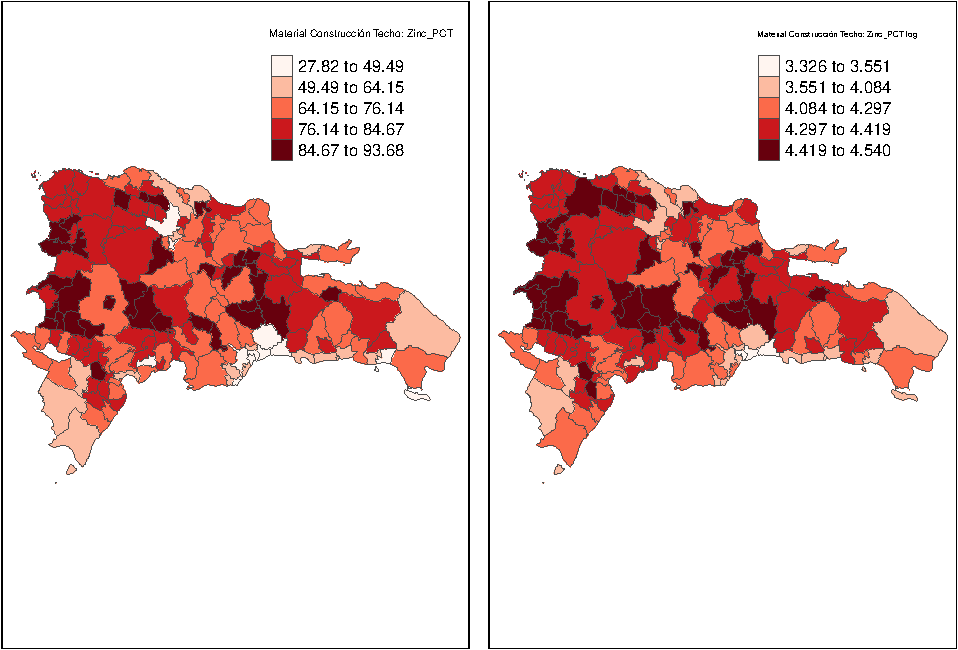
\includegraphics{proyecto_files/figure-latex/unnamed-chunk-2-6.pdf}

\begin{Shaded}
\begin{Highlighting}[]
\NormalTok{vivref }\OperatorTok\StringTok{ }\KeywordTok{st_drop_geometry}\NormalTok{() }\OperatorTok
\StringTok{  }\KeywordTok{select}\NormalTok{(}\KeywordTok{contains}\NormalTok{(}\StringTok{'PCT'}\NormalTok{)) }\OperatorTok\StringTok{ }
\StringTok{  }\KeywordTok{gather}\NormalTok{(variable, valor) }\OperatorTok
\StringTok{  }\KeywordTok{ggplot}\NormalTok{() }\OperatorTok{+}\StringTok{ }\KeywordTok{aes}\NormalTok{(}\DataTypeTok{sample=}\NormalTok{valor) }\OperatorTok{+}
\StringTok{  }\KeywordTok{stat_qq}\NormalTok{() }\OperatorTok{+}\StringTok{ }\KeywordTok{stat_qq_line}\NormalTok{() }\OperatorTok{+}\StringTok{ }\KeywordTok{theme_bw}\NormalTok{() }\OperatorTok{+}
\StringTok{  }\KeywordTok{theme}\NormalTok{(}\DataTypeTok{text =} \KeywordTok{element_text}\NormalTok{(}\DataTypeTok{size =} \DecValTok{14}\NormalTok{)) }\OperatorTok{+}
\StringTok{  }\KeywordTok{facet_wrap}\NormalTok{(}\OperatorTok{~}\NormalTok{variable, }\DataTypeTok{scales =} \StringTok{'free'}\NormalTok{)}
\end{Highlighting}
\end{Shaded}

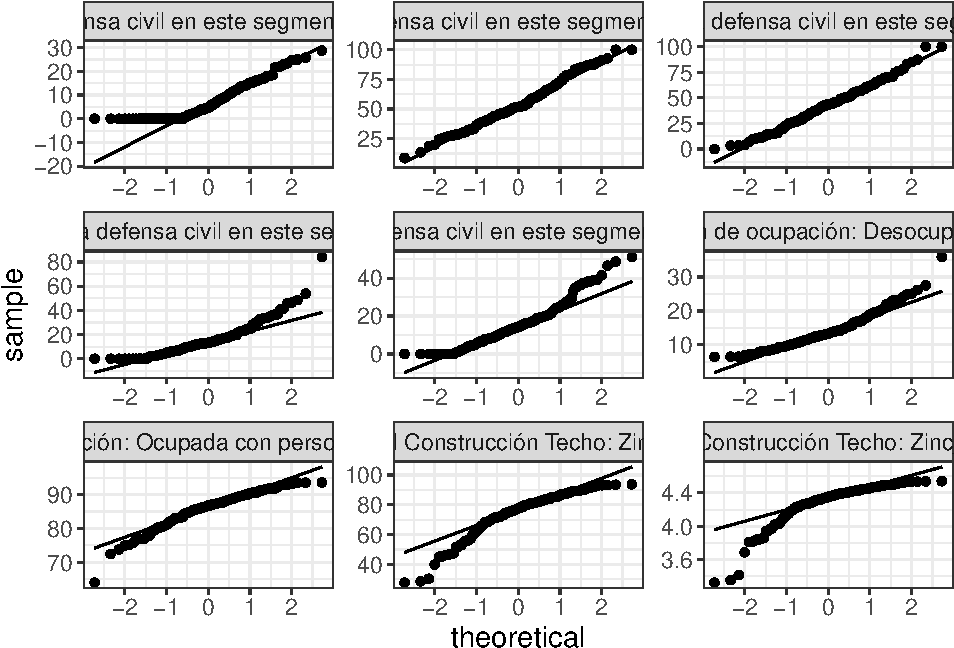
\includegraphics{proyecto_files/figure-latex/unnamed-chunk-2-7.pdf}

\begin{Shaded}
\begin{Highlighting}[]
\NormalTok{vivref }\OperatorTok\StringTok{ }\KeywordTok{st_drop_geometry}\NormalTok{() }\OperatorTok
\StringTok{  }\KeywordTok{gather}\NormalTok{(variable, valor, }\OperatorTok{-}\NormalTok{(TOPONIMIA)) }\OperatorTok\StringTok{ }\KeywordTok{group_by}\NormalTok{(variable) }\OperatorTok
\StringTok{  }\KeywordTok{summarise}\NormalTok{(}\DataTypeTok{prueba_normalidad=}\KeywordTok{shapiro.test}\NormalTok{(valor)}\OperatorTok{$}\NormalTok{p.value)}
\end{Highlighting}
\end{Shaded}

\begin{verbatim}
## # A tibble: 18 x 2
##    variable                                                prueba_normalid~
##    <chr>                                                              <dbl>
##  1 Centros de refugio de la defensa civil en este segment~         2.37e-24
##  2 Centros de refugio de la defensa civil en este segment~         6.20e-10
##  3 Centros de refugio de la defensa civil en este segment~         1.05e-22
##  4 Centros de refugio de la defensa civil en este segment~         1.95e- 1
##  5 Centros de refugio de la defensa civil en este segment~         8.53e-23
##  6 Centros de refugio de la defensa civil en este segment~         4.45e- 1
##  7 Centros de refugio de la defensa civil en este segment~         2.57e-23
##  8 Centros de refugio de la defensa civil en este segment~         4.91e-10
##  9 Centros de refugio de la defensa civil en este segment~         5.28e-23
## 10 Centros de refugio de la defensa civil en este segment~         3.08e- 6
## 11 Condición de ocupación: Desocupada                              6.52e-23
## 12 Condición de ocupación: Desocupada_PCT                          1.60e- 6
## 13 Condición de ocupación: Ocupada con personas presentes          1.13e-22
## 14 Condición de ocupación: Ocupada con personas presentes~         1.60e- 6
## 15 Material Construcción Techo: Zinc                               1.22e-19
## 16 Material Construcción Techo: Zinc_PCT                           1.31e- 8
## 17 Material Construcción Techo: Zinc_PCT log                       3.38e-13
## 18 Total de viviendas                                              1.04e-22
\end{verbatim}

\begin{Shaded}
\begin{Highlighting}[]
\KeywordTok{qqnorm}\NormalTok{(vivref}\OperatorTok{$}\StringTok{`}\DataTypeTok{Material Construcción Techo: Zinc_PCT}\StringTok{`}\NormalTok{)}
\end{Highlighting}
\end{Shaded}

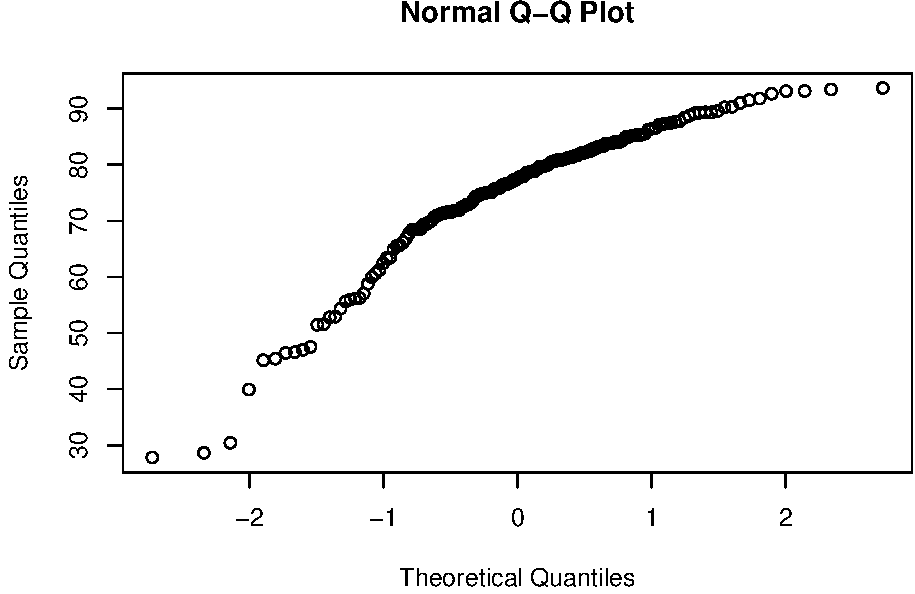
\includegraphics{proyecto_files/figure-latex/unnamed-chunk-2-8.pdf}

\begin{Shaded}
\begin{Highlighting}[]
\KeywordTok{shapiro.test}\NormalTok{(vivref}\OperatorTok{$}\StringTok{`}\DataTypeTok{Material Construcción Techo: Zinc_PCT}\StringTok{`}\NormalTok{) }
\end{Highlighting}
\end{Shaded}

\begin{verbatim}
## 
##  Shapiro-Wilk normality test
## 
## data:  vivref$`Material Construcción Techo: Zinc_PCT`
## W = 0.90313, p-value = 1.314e-08
\end{verbatim}

\begin{Shaded}
\begin{Highlighting}[]
\KeywordTok{qqnorm}\NormalTok{(vivref}\OperatorTok{$}\StringTok{`}\DataTypeTok{Material Construcción Techo: Zinc_PCT log}\StringTok{`}\NormalTok{) }
\end{Highlighting}
\end{Shaded}

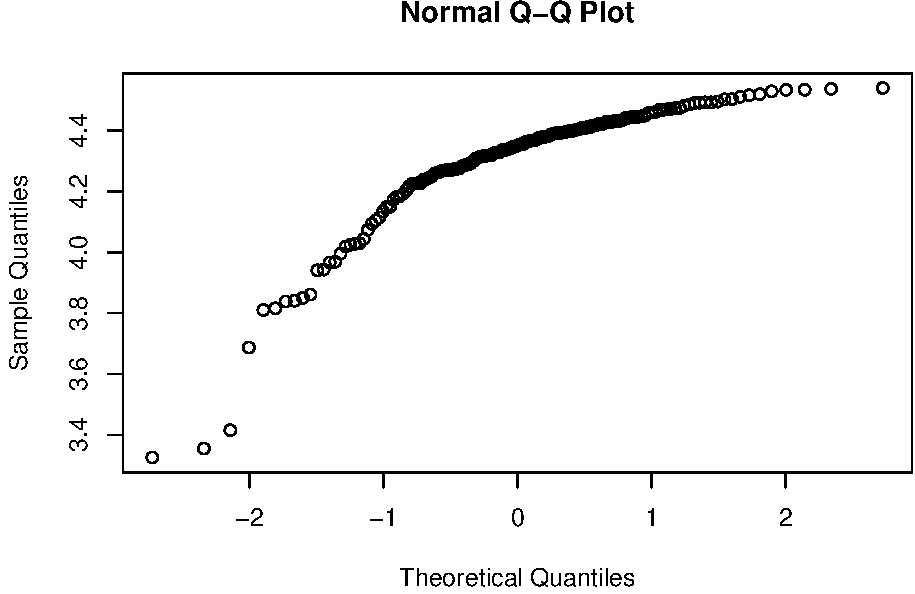
\includegraphics{proyecto_files/figure-latex/unnamed-chunk-2-9.pdf}

\begin{Shaded}
\begin{Highlighting}[]
\KeywordTok{shapiro.test}\NormalTok{(vivref}\OperatorTok{$}\StringTok{`}\DataTypeTok{Material Construcción Techo: Zinc_PCT log}\StringTok{`}\NormalTok{) }
\end{Highlighting}
\end{Shaded}

\begin{verbatim}
## 
##  Shapiro-Wilk normality test
## 
## data:  vivref$`Material Construcción Techo: Zinc_PCT log`
## W = 0.80236, p-value = 3.383e-13
\end{verbatim}

\begin{Shaded}
\begin{Highlighting}[]
\NormalTok{vivrefconxy }\OperatorTok\StringTok{ }\KeywordTok{lm}\NormalTok{(}\StringTok{`}\DataTypeTok{Material Construcción Techo: Zinc_PCT}\StringTok{`}\OperatorTok{~}\NormalTok{x,.) }\OperatorTok\StringTok{ }\KeywordTok{plot}\NormalTok{(}\DecValTok{3}\NormalTok{)}
\end{Highlighting}
\end{Shaded}

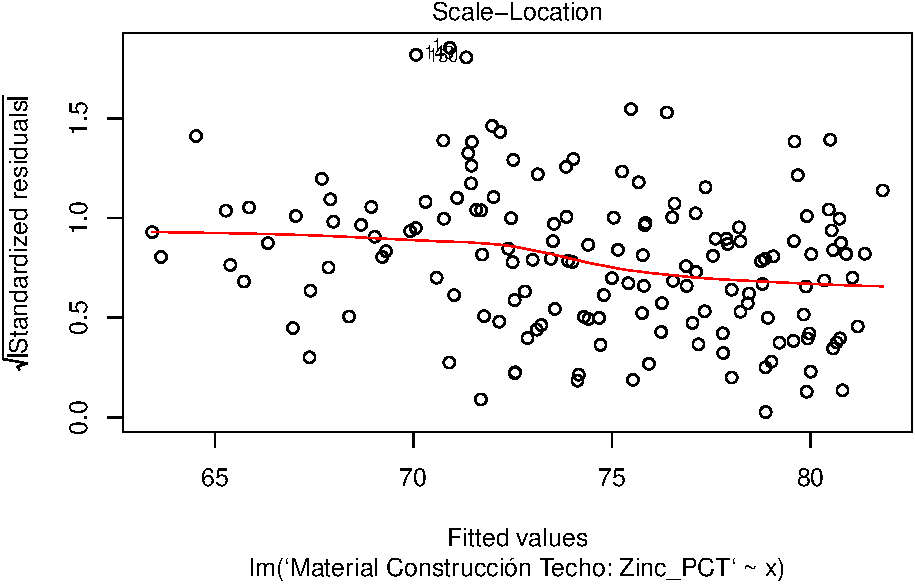
\includegraphics{proyecto_files/figure-latex/unnamed-chunk-2-10.pdf}

\begin{Shaded}
\begin{Highlighting}[]
\NormalTok{vivrefconxy }\OperatorTok\StringTok{ }\KeywordTok{lm}\NormalTok{(}\StringTok{`}\DataTypeTok{Material Construcción Techo: Zinc_PCT}\StringTok{`}\OperatorTok{~}\NormalTok{y,.) }\OperatorTok\StringTok{ }\KeywordTok{plot}\NormalTok{(}\DecValTok{3}\NormalTok{)}
\end{Highlighting}
\end{Shaded}

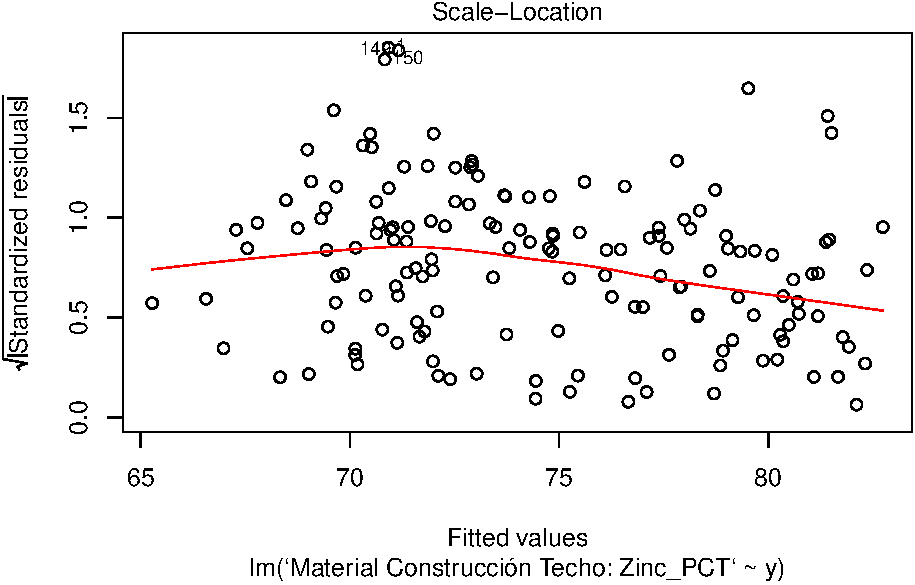
\includegraphics{proyecto_files/figure-latex/unnamed-chunk-2-11.pdf}

\begin{Shaded}
\begin{Highlighting}[]
\NormalTok{vivrefconxy }\OperatorTok\StringTok{ }\KeywordTok{lm}\NormalTok{(}\StringTok{`}\DataTypeTok{Material Construcción Techo: Zinc_PCT log}\StringTok{`}\OperatorTok{~}\NormalTok{x,.) }\OperatorTok\StringTok{ }\KeywordTok{plot}\NormalTok{(}\DecValTok{3}\NormalTok{)}
\end{Highlighting}
\end{Shaded}

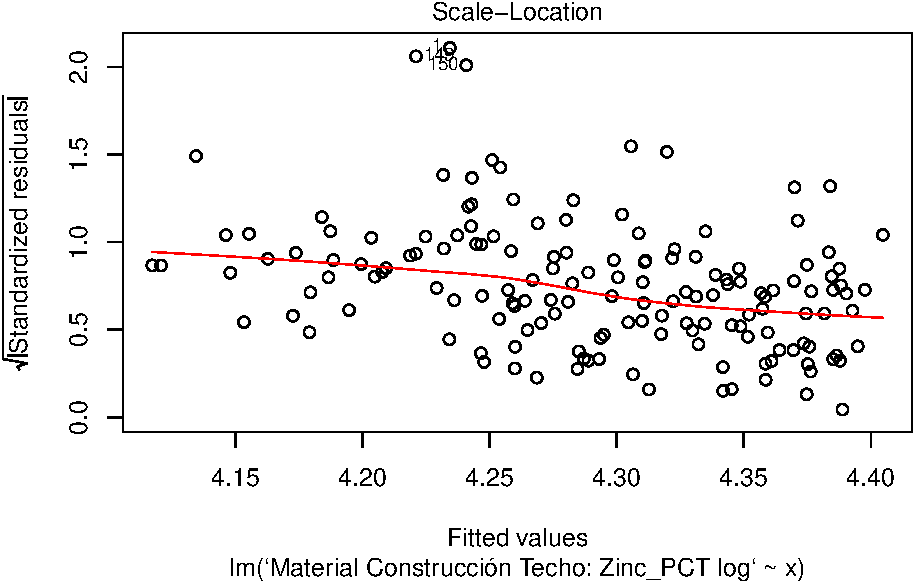
\includegraphics{proyecto_files/figure-latex/unnamed-chunk-2-12.pdf}

\begin{Shaded}
\begin{Highlighting}[]
\NormalTok{vivrefconxy }\OperatorTok\StringTok{ }\KeywordTok{lm}\NormalTok{(}\StringTok{`}\DataTypeTok{Material Construcción Techo: Zinc_PCT log}\StringTok{`}\OperatorTok{~}\NormalTok{y,.) }\OperatorTok\StringTok{ }\KeywordTok{plot}\NormalTok{(}\DecValTok{3}\NormalTok{)}
\end{Highlighting}
\end{Shaded}

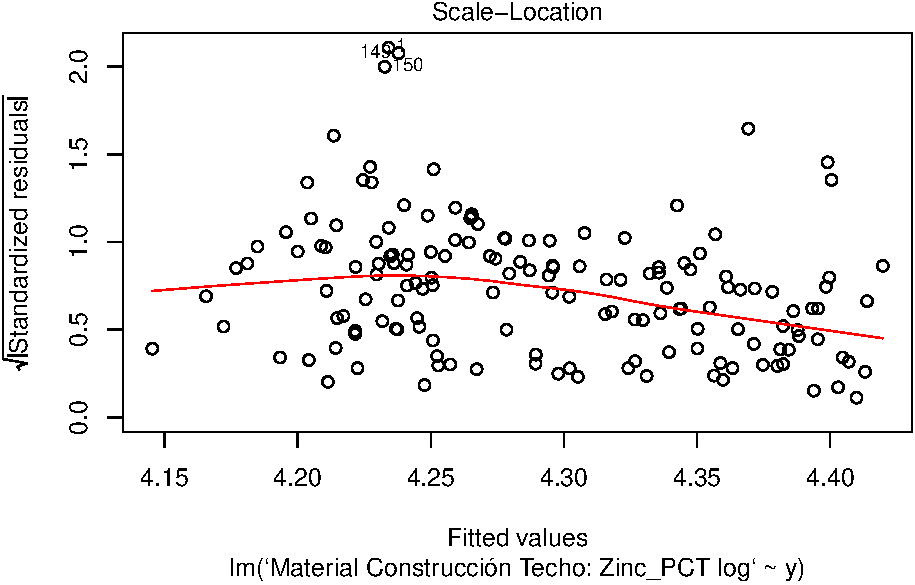
\includegraphics{proyecto_files/figure-latex/unnamed-chunk-2-13.pdf}

\begin{Shaded}
\begin{Highlighting}[]
\KeywordTok{match}\NormalTok{(}\KeywordTok{attr}\NormalTok{(vivref.w.W}\OperatorTok{$}\NormalTok{neighbours, }\StringTok{"region.id"}\NormalTok{), vivref}\OperatorTok{$}\NormalTok{TOPONIMIA)}\OperatorTok{==}\DecValTok{1}\OperatorTok{:}\DecValTok{155}
\end{Highlighting}
\end{Shaded}

\begin{verbatim}
##   [1] TRUE TRUE TRUE TRUE TRUE TRUE TRUE TRUE TRUE TRUE TRUE TRUE TRUE TRUE
##  [15] TRUE TRUE TRUE TRUE TRUE TRUE TRUE TRUE TRUE TRUE TRUE TRUE TRUE TRUE
##  [29] TRUE TRUE TRUE TRUE TRUE TRUE TRUE TRUE TRUE TRUE TRUE TRUE TRUE TRUE
##  [43] TRUE TRUE TRUE TRUE TRUE TRUE TRUE TRUE TRUE TRUE TRUE TRUE TRUE TRUE
##  [57] TRUE TRUE TRUE TRUE TRUE TRUE TRUE TRUE TRUE TRUE TRUE TRUE TRUE TRUE
##  [71] TRUE TRUE TRUE TRUE TRUE TRUE TRUE TRUE TRUE TRUE TRUE TRUE TRUE TRUE
##  [85] TRUE TRUE TRUE TRUE TRUE TRUE TRUE TRUE TRUE TRUE TRUE TRUE TRUE TRUE
##  [99] TRUE TRUE TRUE TRUE TRUE TRUE TRUE TRUE TRUE TRUE TRUE TRUE TRUE TRUE
## [113] TRUE TRUE TRUE TRUE TRUE TRUE TRUE TRUE TRUE TRUE TRUE TRUE TRUE TRUE
## [127] TRUE TRUE TRUE TRUE TRUE TRUE TRUE TRUE TRUE TRUE TRUE TRUE TRUE TRUE
## [141] TRUE TRUE TRUE TRUE TRUE TRUE TRUE TRUE TRUE TRUE TRUE TRUE TRUE TRUE
## [155] TRUE
\end{verbatim}

\begin{Shaded}
\begin{Highlighting}[]
\NormalTok{(gmoranw <-}\StringTok{ }\KeywordTok{moran.test}\NormalTok{(}\DataTypeTok{x =}\NormalTok{ vivref}\OperatorTok{$}\StringTok{`}\DataTypeTok{Material Construcción Techo: Zinc_PCT log}\StringTok{`}\NormalTok{, }\DataTypeTok{listw =}\NormalTok{ vivref.w.W))}
\end{Highlighting}
\end{Shaded}

\begin{verbatim}
## 
##  Moran I test under randomisation
## 
## data:  vivref$`Material Construcción Techo: Zinc_PCT log`  
## weights: vivref.w.W    
## 
## Moran I statistic standard deviate = 9.7935, p-value < 2.2e-16
## alternative hypothesis: greater
## sample estimates:
## Moran I statistic       Expectation          Variance 
##       0.488809637      -0.006493506       0.002557784
\end{verbatim}

\begin{Shaded}
\begin{Highlighting}[]
\NormalTok{(gmoranb <-}\StringTok{ }\KeywordTok{moran.test}\NormalTok{(}\DataTypeTok{x =}\NormalTok{ vivref}\OperatorTok{$}\StringTok{`}\DataTypeTok{Material Construcción Techo: Zinc_PCT log}\StringTok{`}\NormalTok{, }\DataTypeTok{listw =}\NormalTok{ vivref.w.B))}
\end{Highlighting}
\end{Shaded}

\begin{verbatim}
## 
##  Moran I test under randomisation
## 
## data:  vivref$`Material Construcción Techo: Zinc_PCT log`  
## weights: vivref.w.B    
## 
## Moran I statistic standard deviate = 8.884, p-value < 2.2e-16
## alternative hypothesis: greater
## sample estimates:
## Moran I statistic       Expectation          Variance 
##       0.418744111      -0.006493506       0.002291090
\end{verbatim}

\begin{Shaded}
\begin{Highlighting}[]
\KeywordTok{moran.plot}\NormalTok{(}\DataTypeTok{x =}\NormalTok{ vivref}\OperatorTok{$}\StringTok{`}\DataTypeTok{Material Construcción Techo: Zinc_PCT log}\StringTok{`}\NormalTok{, }\DataTypeTok{listw =}\NormalTok{ vivref.w.W)}
\end{Highlighting}
\end{Shaded}

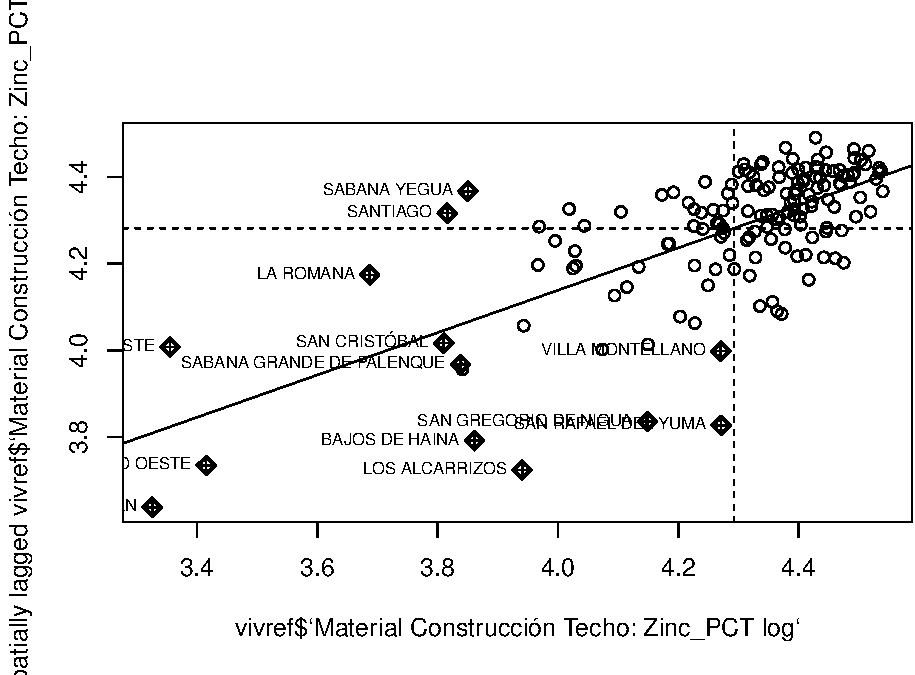
\includegraphics{proyecto_files/figure-latex/unnamed-chunk-2-14.pdf}

\begin{Shaded}
\begin{Highlighting}[]
\KeywordTok{source}\NormalTok{(}\StringTok{'lisaclusters.R'}\NormalTok{)}
\KeywordTok{lisamap}\NormalTok{(}\DataTypeTok{objesp=}\NormalTok{vivref,}
        \DataTypeTok{var =} \StringTok{'Material Construcción Techo: Zinc_PCT'}\NormalTok{,}
        \DataTypeTok{pesos =}\NormalTok{ vivref.w.W,}
        \DataTypeTok{tituloleyenda =} \StringTok{'Significancia}\CharTok{\textbackslash{}n}\StringTok{("x-y", léase}\CharTok{\textbackslash{}n}\StringTok{como "x"}\CharTok{\textbackslash{}n}\StringTok{rodeado de "y"'}\NormalTok{,}
        \DataTypeTok{leyenda =}\NormalTok{ T,}
        \DataTypeTok{anchuratitulo =} \DecValTok{1000}\NormalTok{,}
        \DataTypeTok{tamanotitulo =} \DecValTok{16}\NormalTok{,}
        \DataTypeTok{fuentedatos =}\StringTok{'CENSO 2010'}\NormalTok{,}
        \DataTypeTok{titulomapa =} \KeywordTok{paste0}\NormalTok{(}\StringTok{'Clusters LISA, de la variable Total de viviendas'}\NormalTok{))}
\end{Highlighting}
\end{Shaded}

\begin{verbatim}
## $grafico
\end{verbatim}

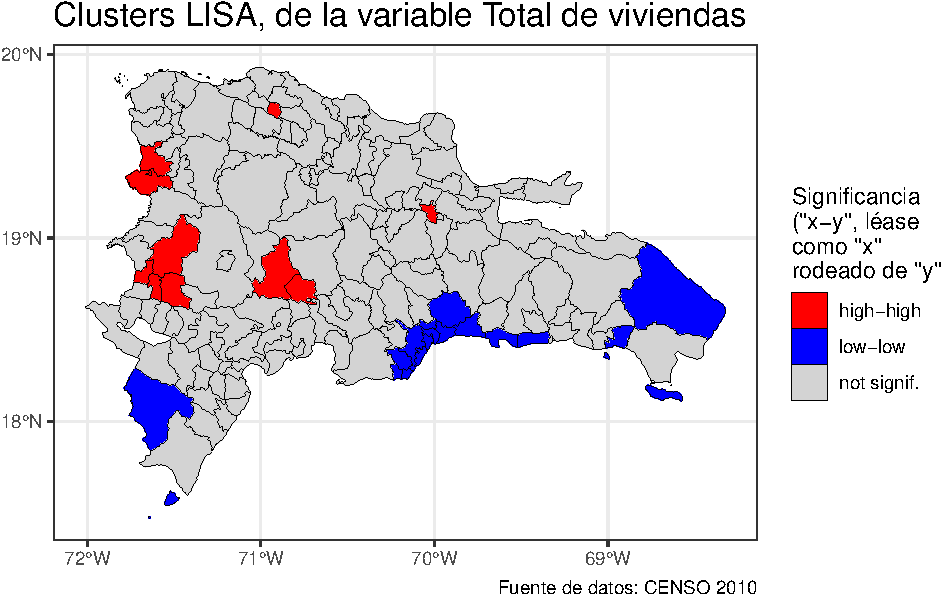
\includegraphics{proyecto_files/figure-latex/unnamed-chunk-2-15.pdf}

\begin{verbatim}
## 
## $objeto
## Simple feature collection with 155 features and 22 fields
## geometry type:  MULTIPOLYGON
## dimension:      XY
## bbox:           xmin: -72.01147 ymin: 17.47033 xmax: -68.32354 ymax: 19.93211
## epsg (SRID):    4326
## proj4string:    +proj=longlat +datum=WGS84 +no_defs
## First 10 features:
##                  TOPONIMIA
## 1  SANTO DOMINGO DE GUZMÁN
## 2                     AZUA
## 3              LAS CHARCAS
## 4     LAS YAYAS DE VIAJAMA
## 5          PADRE LAS CASAS
## 6                  PERALTA
## 7             SABANA YEGUA
## 8             PUEBLO VIEJO
## 9            TÁBARA ARRIBA
## 10                GUAYABAL
##    Condición de ocupación: Ocupada con personas presentes
## 1                                                  288362
## 2                                                   22797
## 3                                                    3147
## 4                                                    4807
## 5                                                    5243
## 6                                                    3144
## 7                                                    4828
## 8                                                    2689
## 9                                                    4108
## 10                                                   1386
##    Condición de ocupación: Desocupada Material Construcción Techo: Zinc
## 1                               42200                             91950
## 2                                1920                             18544
## 3                                 944                              2919
## 4                                 798                              4475
## 5                                1345                              5874
## 6                                 446                              3019
## 7                                 594                              2549
## 8                                 208                              2294
## 9                                 426                              3737
## 10                                464                              1723
##    Centros de refugio de la defensa civil en este segmento: Escuela o Liceo: Si
## 1                                                                        174938
## 2                                                                         12706
## 3                                                                           763
## 4                                                                          3722
## 5                                                                          3400
## 6                                                                          2458
## 7                                                                          3206
## 8                                                                          2266
## 9                                                                          2239
## 10                                                                         1584
##    Centros de refugio de la defensa civil en este segmento: Iglesia: Si
## 1                                                                170337
## 2                                                                  9122
## 3                                                                   425
## 4                                                                  3421
## 5                                                                  1422
## 6                                                                   684
## 7                                                                   196
## 8                                                                    99
## 9                                                                   319
## 10                                                                  290
##    Centros de refugio de la defensa civil en este segmento: Salón comunal: Si
## 1                                                                       61706
## 2                                                                        4718
## 3                                                                           0
## 4                                                                         229
## 5                                                                         790
## 6                                                                         999
## 7                                                                          59
## 8                                                                         698
## 9                                                                         371
## 10                                                                          0
##    Centros de refugio de la defensa civil en este segmento: Centro deportivo: Si
## 1                                                                          77246
## 2                                                                           2525
## 3                                                                              0
## 4                                                                             52
## 5                                                                            434
## 6                                                                            262
## 7                                                                            969
## 8                                                                              0
## 9                                                                            178
## 10                                                                             0
##    Centros de refugio de la defensa civil en este segmento: Otros: Si
## 1                                                               71189
## 2                                                                4565
## 3                                                                   0
## 4                                                                 560
## 5                                                                1284
## 6                                                                1206
## 7                                                                2480
## 8                                                                   0
## 9                                                                 574
## 10                                                                679
##                              geom Total de viviendas
## 1  MULTIPOLYGON (((-69.89794 1...             330562
## 2  MULTIPOLYGON (((-70.71457 1...              24717
## 3  MULTIPOLYGON (((-70.50185 1...               4091
## 4  MULTIPOLYGON (((-70.85774 1...               5605
## 5  MULTIPOLYGON (((-70.77551 1...               6588
## 6  MULTIPOLYGON (((-70.73131 1...               3590
## 7  MULTIPOLYGON (((-70.83014 1...               5422
## 8  MULTIPOLYGON (((-70.79387 1...               2897
## 9  MULTIPOLYGON (((-70.83352 1...               4534
## 10 MULTIPOLYGON (((-70.68664 1...               1850
##    Condición de ocupación: Ocupada con personas presentes_PCT
## 1                                                       87.23
## 2                                                       92.23
## 3                                                       76.92
## 4                                                       85.76
## 5                                                       79.58
## 6                                                       87.58
## 7                                                       89.04
## 8                                                       92.82
## 9                                                       90.60
## 10                                                      74.92
##    Condición de ocupación: Desocupada_PCT
## 1                                   12.77
## 2                                    7.77
## 3                                   23.08
## 4                                   14.24
## 5                                   20.42
## 6                                   12.42
## 7                                   10.96
## 8                                    7.18
## 9                                    9.40
## 10                                  25.08
##    Material Construcción Techo: Zinc_PCT
## 1                                  27.82
## 2                                  75.03
## 3                                  71.35
## 4                                  79.84
## 5                                  89.16
## 6                                  84.09
## 7                                  47.01
## 8                                  79.19
## 9                                  82.42
## 10                                 93.14
##    Centros de refugio de la defensa civil en este segmento: Escuela o Liceo: Si_PCT
## 1                                                                             52.92
## 2                                                                             51.41
## 3                                                                             18.65
## 4                                                                             66.40
## 5                                                                             51.61
## 6                                                                             68.47
## 7                                                                             59.13
## 8                                                                             78.22
## 9                                                                             49.38
## 10                                                                            85.62
##    Centros de refugio de la defensa civil en este segmento: Iglesia: Si_PCT
## 1                                                                     51.53
## 2                                                                     36.91
## 3                                                                     10.39
## 4                                                                     61.03
## 5                                                                     21.58
## 6                                                                     19.05
## 7                                                                      3.61
## 8                                                                      3.42
## 9                                                                      7.04
## 10                                                                    15.68
##    Centros de refugio de la defensa civil en este segmento: Salón comunal: Si_PCT
## 1                                                                           18.67
## 2                                                                           19.09
## 3                                                                            0.00
## 4                                                                            4.09
## 5                                                                           11.99
## 6                                                                           27.83
## 7                                                                            1.09
## 8                                                                           24.09
## 9                                                                            8.18
## 10                                                                           0.00
##    Centros de refugio de la defensa civil en este segmento: Centro deportivo: Si_PCT
## 1                                                                              23.37
## 2                                                                              10.22
## 3                                                                               0.00
## 4                                                                               0.93
## 5                                                                               6.59
## 6                                                                               7.30
## 7                                                                              17.87
## 8                                                                               0.00
## 9                                                                               3.93
## 10                                                                              0.00
##    Centros de refugio de la defensa civil en este segmento: Otros: Si_PCT
## 1                                                                   21.54
## 2                                                                   18.47
## 3                                                                    0.00
## 4                                                                    9.99
## 5                                                                   19.49
## 6                                                                   33.59
## 7                                                                   45.74
## 8                                                                    0.00
## 9                                                                   12.66
## 10                                                                  36.70
##    Material Construcción Techo: Zinc_PCT log puntuacionz lagpuntuacionz
## 1                                   3.325755 -3.51642931    -2.65555077
## 2                                   4.317888  0.02999965    -0.16681551
## 3                                   4.267597 -0.24644302    -0.08869041
## 4                                   4.380025  0.39132825     0.30544072
## 5                                   4.490433  1.09144937     0.56861214
## 6                                   4.431888  0.71058949     0.66263771
## 7                                   3.850360 -2.07487091     0.31921277
## 8                                   4.371850  0.34250006    -1.02243563
## 9                                   4.411828  0.58513861    -0.39918761
## 10                                  4.534104  1.39042813     0.58513861
##       quad_sig
## 1      low-low
## 2  not signif.
## 3  not signif.
## 4  not signif.
## 5    high-high
## 6  not signif.
## 7  not signif.
## 8  not signif.
## 9  not signif.
## 10   high-high
\end{verbatim}

\begin{Shaded}
\begin{Highlighting}[]
\CommentTok{# MODELIZACION}

\NormalTok{varsel <-}\StringTok{ }\NormalTok{vivref }\OperatorTok\StringTok{ }\NormalTok{dplyr}\OperatorTok{::}\KeywordTok{select}\NormalTok{(}
  \DataTypeTok{TOPONIMIA =}\NormalTok{ TOPONIMIA,}
  \DataTypeTok{TECHOZINC =} \StringTok{`}\DataTypeTok{Material Construcción Techo: Zinc_PCT}\StringTok{`}\NormalTok{,}
  \DataTypeTok{CENTROEDU =} \StringTok{`}\DataTypeTok{Centros de refugio de la defensa civil en este segmento: Escuela o Liceo: Si_PCT}\StringTok{`}\NormalTok{,}
  \DataTypeTok{CENTROREL =} \StringTok{`}\DataTypeTok{Centros de refugio de la defensa civil en este segmento: Iglesia: Si_PCT}\StringTok{`}\NormalTok{,}
  \DataTypeTok{SALONCOMU =} \StringTok{`}\DataTypeTok{Centros de refugio de la defensa civil en este segmento: Salón comunal: Si_PCT}\StringTok{`}\NormalTok{,}
  \DataTypeTok{DEPORTIVO =} \StringTok{`}\DataTypeTok{Centros de refugio de la defensa civil en este segmento: Centro deportivo: Si_PCT}\StringTok{`}\NormalTok{,}
  \DataTypeTok{DEFENSACIV=} \StringTok{`}\DataTypeTok{Centros de refugio de la defensa civil en este segmento: Otros: Si_PCT}\StringTok{`}\NormalTok{,}
  \DataTypeTok{TOTALVIV =} \StringTok{`}\DataTypeTok{Total de viviendas}\StringTok{`}\NormalTok{)}
\NormalTok{varsel}
\end{Highlighting}
\end{Shaded}

\begin{verbatim}
## Simple feature collection with 155 features and 8 fields
## geometry type:  MULTIPOLYGON
## dimension:      XY
## bbox:           xmin: -72.01147 ymin: 17.47033 xmax: -68.32354 ymax: 19.93211
## epsg (SRID):    4326
## proj4string:    +proj=longlat +datum=WGS84 +no_defs
## First 10 features:
##                  TOPONIMIA TECHOZINC CENTROEDU CENTROREL SALONCOMU
## 1  SANTO DOMINGO DE GUZMÁN     27.82     52.92     51.53     18.67
## 2                     AZUA     75.03     51.41     36.91     19.09
## 3              LAS CHARCAS     71.35     18.65     10.39      0.00
## 4     LAS YAYAS DE VIAJAMA     79.84     66.40     61.03      4.09
## 5          PADRE LAS CASAS     89.16     51.61     21.58     11.99
## 6                  PERALTA     84.09     68.47     19.05     27.83
## 7             SABANA YEGUA     47.01     59.13      3.61      1.09
## 8             PUEBLO VIEJO     79.19     78.22      3.42     24.09
## 9            TÁBARA ARRIBA     82.42     49.38      7.04      8.18
## 10                GUAYABAL     93.14     85.62     15.68      0.00
##    DEPORTIVO DEFENSACIV TOTALVIV                           geom
## 1      23.37      21.54   330562 MULTIPOLYGON (((-69.89794 1...
## 2      10.22      18.47    24717 MULTIPOLYGON (((-70.71457 1...
## 3       0.00       0.00     4091 MULTIPOLYGON (((-70.50185 1...
## 4       0.93       9.99     5605 MULTIPOLYGON (((-70.85774 1...
## 5       6.59      19.49     6588 MULTIPOLYGON (((-70.77551 1...
## 6       7.30      33.59     3590 MULTIPOLYGON (((-70.73131 1...
## 7      17.87      45.74     5422 MULTIPOLYGON (((-70.83014 1...
## 8       0.00       0.00     2897 MULTIPOLYGON (((-70.79387 1...
## 9       3.93      12.66     4534 MULTIPOLYGON (((-70.83352 1...
## 10      0.00      36.70     1850 MULTIPOLYGON (((-70.68664 1...
\end{verbatim}

\begin{Shaded}
\begin{Highlighting}[]
\NormalTok{varselpctlog <-}\StringTok{ }\NormalTok{varsel }\OperatorTok\StringTok{ }\KeywordTok{mutate_each}\NormalTok{(}
  \KeywordTok{funs}\NormalTok{(}\DataTypeTok{PCT=}\KeywordTok{round}\NormalTok{(.}\OperatorTok{/}\NormalTok{TOTALVIV,}\DecValTok{4}\NormalTok{)}\OperatorTok{*}\DecValTok{100}\NormalTok{,}
       \DataTypeTok{PCTLOG=}\KeywordTok{log1p}\NormalTok{(}\KeywordTok{round}\NormalTok{(.}\OperatorTok{/}\NormalTok{TOTALVIV,}\DecValTok{4}\NormalTok{)}\OperatorTok{*}\DecValTok{100}\NormalTok{)),}
  \OperatorTok{-}\DecValTok{1}\NormalTok{, }\OperatorTok{-}\DecValTok{2}\NormalTok{, }\OperatorTok{-}\NormalTok{geom, }\OperatorTok{-}\NormalTok{TOTALVIV)}
\NormalTok{varselpctlog}
\end{Highlighting}
\end{Shaded}

\begin{verbatim}
## Simple feature collection with 155 features and 18 fields
## geometry type:  MULTIPOLYGON
## dimension:      XY
## bbox:           xmin: -72.01147 ymin: 17.47033 xmax: -68.32354 ymax: 19.93211
## epsg (SRID):    4326
## proj4string:    +proj=longlat +datum=WGS84 +no_defs
## First 10 features:
##                  TOPONIMIA TECHOZINC CENTROEDU CENTROREL SALONCOMU
## 1  SANTO DOMINGO DE GUZMÁN     27.82     52.92     51.53     18.67
## 2                     AZUA     75.03     51.41     36.91     19.09
## 3              LAS CHARCAS     71.35     18.65     10.39      0.00
## 4     LAS YAYAS DE VIAJAMA     79.84     66.40     61.03      4.09
## 5          PADRE LAS CASAS     89.16     51.61     21.58     11.99
## 6                  PERALTA     84.09     68.47     19.05     27.83
## 7             SABANA YEGUA     47.01     59.13      3.61      1.09
## 8             PUEBLO VIEJO     79.19     78.22      3.42     24.09
## 9            TÁBARA ARRIBA     82.42     49.38      7.04      8.18
## 10                GUAYABAL     93.14     85.62     15.68      0.00
##    DEPORTIVO DEFENSACIV TOTALVIV                           geom
## 1      23.37      21.54   330562 MULTIPOLYGON (((-69.89794 1...
## 2      10.22      18.47    24717 MULTIPOLYGON (((-70.71457 1...
## 3       0.00       0.00     4091 MULTIPOLYGON (((-70.50185 1...
## 4       0.93       9.99     5605 MULTIPOLYGON (((-70.85774 1...
## 5       6.59      19.49     6588 MULTIPOLYGON (((-70.77551 1...
## 6       7.30      33.59     3590 MULTIPOLYGON (((-70.73131 1...
## 7      17.87      45.74     5422 MULTIPOLYGON (((-70.83014 1...
## 8       0.00       0.00     2897 MULTIPOLYGON (((-70.79387 1...
## 9       3.93      12.66     4534 MULTIPOLYGON (((-70.83352 1...
## 10      0.00      36.70     1850 MULTIPOLYGON (((-70.68664 1...
##    CENTROEDU_PCT CENTROREL_PCT SALONCOMU_PCT DEPORTIVO_PCT DEFENSACIV_PCT
## 1           0.02          0.02          0.01          0.01           0.01
## 2           0.21          0.15          0.08          0.04           0.07
## 3           0.46          0.25          0.00          0.00           0.00
## 4           1.18          1.09          0.07          0.02           0.18
## 5           0.78          0.33          0.18          0.10           0.30
## 6           1.91          0.53          0.78          0.20           0.94
## 7           1.09          0.07          0.02          0.33           0.84
## 8           2.70          0.12          0.83          0.00           0.00
## 9           1.09          0.16          0.18          0.09           0.28
## 10          4.63          0.85          0.00          0.00           1.98
##    CENTROEDU_PCTLOG CENTROREL_PCTLOG SALONCOMU_PCTLOG DEPORTIVO_PCTLOG
## 1        0.01980263       0.01980263      0.009950331      0.009950331
## 2        0.19062036       0.13976194      0.076961041      0.039220713
## 3        0.37843644       0.22314355      0.000000000      0.000000000
## 4        0.77932488       0.73716407      0.067658648      0.019802627
## 5        0.57661336       0.28517894      0.165514438      0.095310180
## 6        1.06815308       0.42526774      0.576613364      0.182321557
## 7        0.73716407       0.06765865      0.019802627      0.285178942
## 8        1.30833282       0.11332869      0.604315967      0.000000000
## 9        0.73716407       0.14842001      0.165514438      0.086177696
## 10       1.72810944       0.61518564      0.000000000      0.000000000
##    DEFENSACIV_PCTLOG
## 1        0.009950331
## 2        0.067658648
## 3        0.000000000
## 4        0.165514438
## 5        0.262364264
## 6        0.662687973
## 7        0.609765572
## 8        0.000000000
## 9        0.246860078
## 10       1.091923301
\end{verbatim}

\begin{Shaded}
\begin{Highlighting}[]
\NormalTok{(gmoranw <-}\StringTok{ }\KeywordTok{moran.test}\NormalTok{(}\DataTypeTok{x =}\NormalTok{ varselpctlog}\OperatorTok{$}\NormalTok{CENTROEDU_PCT, }\DataTypeTok{listw =}\NormalTok{ vivref.w.W))}
\end{Highlighting}
\end{Shaded}

\begin{verbatim}
## 
##  Moran I test under randomisation
## 
## data:  varselpctlog$CENTROEDU_PCT  
## weights: vivref.w.W    
## 
## Moran I statistic standard deviate = 5.9444, p-value = 1.387e-09
## alternative hypothesis: greater
## sample estimates:
## Moran I statistic       Expectation          Variance 
##       0.291379238      -0.006493506       0.002510992
\end{verbatim}

\begin{Shaded}
\begin{Highlighting}[]
\NormalTok{(gmoranb <-}\StringTok{ }\KeywordTok{moran.test}\NormalTok{(}\DataTypeTok{x =}\NormalTok{ varselpctlog}\OperatorTok{$}\NormalTok{CENTROEDU_PCT, }\DataTypeTok{listw =}\NormalTok{ vivref.w.B))}
\end{Highlighting}
\end{Shaded}

\begin{verbatim}
## 
##  Moran I test under randomisation
## 
## data:  varselpctlog$CENTROEDU_PCT  
## weights: vivref.w.B    
## 
## Moran I statistic standard deviate = 6.282, p-value = 1.671e-10
## alternative hypothesis: greater
## sample estimates:
## Moran I statistic       Expectation          Variance 
##       0.291460634      -0.006493506       0.002249566
\end{verbatim}

\begin{Shaded}
\begin{Highlighting}[]
\NormalTok{(gmoranwl <-}\StringTok{ }\KeywordTok{moran.test}\NormalTok{(}\DataTypeTok{x =}\NormalTok{ varselpctlog}\OperatorTok{$}\NormalTok{CENTROEDU_PCTLOG, }\DataTypeTok{listw =}\NormalTok{ vivref.w.W))}
\end{Highlighting}
\end{Shaded}

\begin{verbatim}
## 
##  Moran I test under randomisation
## 
## data:  varselpctlog$CENTROEDU_PCTLOG  
## weights: vivref.w.W    
## 
## Moran I statistic standard deviate = 6.5511, p-value = 2.855e-11
## alternative hypothesis: greater
## sample estimates:
## Moran I statistic       Expectation          Variance 
##       0.330116769      -0.006493506       0.002640099
\end{verbatim}

\begin{Shaded}
\begin{Highlighting}[]
\NormalTok{(gmoranbl <-}\StringTok{ }\KeywordTok{moran.test}\NormalTok{(}\DataTypeTok{x =}\NormalTok{ varselpctlog}\OperatorTok{$}\NormalTok{CENTROEDU_PCTLOG, }\DataTypeTok{listw =}\NormalTok{ vivref.w.B))}
\end{Highlighting}
\end{Shaded}

\begin{verbatim}
## 
##  Moran I test under randomisation
## 
## data:  varselpctlog$CENTROEDU_PCTLOG  
## weights: vivref.w.B    
## 
## Moran I statistic standard deviate = 6.9541, p-value = 1.774e-12
## alternative hypothesis: greater
## sample estimates:
## Moran I statistic       Expectation          Variance 
##       0.331630182      -0.006493506       0.002364139
\end{verbatim}

\begin{Shaded}
\begin{Highlighting}[]
\KeywordTok{shapiro.test}\NormalTok{(varselpctlog}\OperatorTok{$}\NormalTok{CENTROEDU_PCT)}
\end{Highlighting}
\end{Shaded}

\begin{verbatim}
## 
##  Shapiro-Wilk normality test
## 
## data:  varselpctlog$CENTROEDU_PCT
## W = 0.71801, p-value = 6.68e-16
\end{verbatim}

\begin{Shaded}
\begin{Highlighting}[]
\KeywordTok{shapiro.test}\NormalTok{(varselpctlog}\OperatorTok{$}\NormalTok{CENTROEDU_PCTLOG)}
\end{Highlighting}
\end{Shaded}

\begin{verbatim}
## 
##  Shapiro-Wilk normality test
## 
## data:  varselpctlog$CENTROEDU_PCTLOG
## W = 0.90973, p-value = 3.251e-08
\end{verbatim}

\begin{Shaded}
\begin{Highlighting}[]
\NormalTok{modlin <-}\StringTok{ }\NormalTok{varselpctlog }\OperatorTok\StringTok{ }\KeywordTok{select}\NormalTok{(}\KeywordTok{contains}\NormalTok{(}\StringTok{'_PCTLOG'}\NormalTok{)) }\OperatorTok
\StringTok{  }\KeywordTok{st_drop_geometry}\NormalTok{() }\OperatorTok\StringTok{ }\KeywordTok{lm}\NormalTok{(CENTROEDU_PCTLOG }\OperatorTok{~}\StringTok{ }\NormalTok{., .)}
\NormalTok{modlin }\OperatorTok\StringTok{ }\NormalTok{summary}
\end{Highlighting}
\end{Shaded}

\begin{verbatim}
## 
## Call:
## lm(formula = CENTROEDU_PCTLOG ~ ., data = .)
## 
## Residuals:
##      Min       1Q   Median       3Q      Max 
## -0.53857 -0.12487 -0.07332  0.08091  1.37992 
## 
## Coefficients:
##                   Estimate Std. Error t value Pr(>|t|)    
## (Intercept)        0.11566    0.03125   3.702  0.00030 ***
## CENTROREL_PCTLOG   0.81542    0.05988  13.618  < 2e-16 ***
## SALONCOMU_PCTLOG   0.07762    0.10009   0.776  0.43924    
## DEPORTIVO_PCTLOG   0.35455    0.18184   1.950  0.05306 .  
## DEFENSACIV_PCTLOG  0.27021    0.08080   3.344  0.00104 ** 
## ---
## Signif. codes:  0 '***' 0.001 '**' 0.01 '*' 0.05 '.' 0.1 ' ' 1
## 
## Residual standard error: 0.2382 on 150 degrees of freedom
## Multiple R-squared:  0.7581, Adjusted R-squared:  0.7517 
## F-statistic: 117.5 on 4 and 150 DF,  p-value: < 2.2e-16
\end{verbatim}

\begin{Shaded}
\begin{Highlighting}[]
\NormalTok{modlin }\OperatorTok\StringTok{ }\NormalTok{bptest}
\end{Highlighting}
\end{Shaded}

\begin{verbatim}
## 
##  studentized Breusch-Pagan test
## 
## data:  .
## BP = 3.7175, df = 4, p-value = 0.4456
\end{verbatim}

\begin{Shaded}
\begin{Highlighting}[]
\CommentTok{# Ejecutemos el modelo espacial autorregresivo, en este caso, la variate Simultaneous Autorregresive Model.}

\NormalTok{sar <-}\StringTok{ }\NormalTok{varselpctlog }\OperatorTok\StringTok{ }\KeywordTok{select}\NormalTok{(}\KeywordTok{contains}\NormalTok{(}\StringTok{'_PCTLOG'}\NormalTok{)) }\OperatorTok
\StringTok{  }\KeywordTok{st_drop_geometry}\NormalTok{() }\OperatorTok
\StringTok{  }\KeywordTok{spautolm}\NormalTok{(}
    \DataTypeTok{formula =}\NormalTok{ CENTROEDU_PCTLOG }\OperatorTok{~}\StringTok{ }\NormalTok{.,}
    \DataTypeTok{data =}\NormalTok{ .,}
    \DataTypeTok{listw =}\NormalTok{ vivref.w.W)}
\end{Highlighting}
\end{Shaded}

\begin{verbatim}
## Warning: Function spautolm moved to the spatialreg package
\end{verbatim}

\begin{verbatim}
## Warning in spautolm(formula = CENTROEDU_PCTLOG ~ ., data = ., listw =
## vivref.w.W): install the spatialreg package
\end{verbatim}

\begin{verbatim}
## Warning: Function can.be.simmed moved to the spatialreg package
\end{verbatim}

\begin{verbatim}
## Warning in can.be.simmed(listw): install the spatialreg package
\end{verbatim}

\begin{verbatim}
## Warning: Function as_dgRMatrix_listw moved to the spatialreg package
\end{verbatim}

\begin{verbatim}
## Warning in as_dgRMatrix_listw(from): install the spatialreg package
\end{verbatim}

\begin{verbatim}
## Warning: Function as_dsCMatrix_I moved to the spatialreg package
\end{verbatim}

\begin{verbatim}
## Warning in as_dsCMatrix_I(n): install the spatialreg package
\end{verbatim}

\begin{verbatim}
## Warning: Function jacobianSetup moved to the spatialreg package
\end{verbatim}

\begin{verbatim}
## Warning in jacobianSetup(method, env, con, pre_eig = con$pre_eig, trs =
## trs, : install the spatialreg package
\end{verbatim}

\begin{verbatim}
## Warning: Function eigen_setup moved to the spatialreg package
\end{verbatim}

\begin{verbatim}
## Warning in eigen_setup(env, which = which): install the spatialreg package
\end{verbatim}

\begin{verbatim}
## Warning: Function as_dgRMatrix_listw moved to the spatialreg package
\end{verbatim}

\begin{verbatim}
## Warning in as_dgRMatrix_listw(from): install the spatialreg package
\end{verbatim}

\begin{verbatim}
## Warning: Function do_ldet moved to the spatialreg package
\end{verbatim}

\begin{verbatim}
## Warning in do_ldet(lambda, env): install the spatialreg package
\end{verbatim}

\begin{verbatim}
## Warning: Function do_ldet moved to the spatialreg package
\end{verbatim}

\begin{verbatim}
## Warning in do_ldet(lambda, env): install the spatialreg package
\end{verbatim}

\begin{verbatim}
## Warning: Function do_ldet moved to the spatialreg package
\end{verbatim}

\begin{verbatim}
## Warning in do_ldet(lambda, env): install the spatialreg package
\end{verbatim}

\begin{verbatim}
## Warning: Function do_ldet moved to the spatialreg package
\end{verbatim}

\begin{verbatim}
## Warning in do_ldet(lambda, env): install the spatialreg package
\end{verbatim}

\begin{verbatim}
## Warning: Function do_ldet moved to the spatialreg package
\end{verbatim}

\begin{verbatim}
## Warning in do_ldet(lambda, env): install the spatialreg package
\end{verbatim}

\begin{verbatim}
## Warning: Function do_ldet moved to the spatialreg package
\end{verbatim}

\begin{verbatim}
## Warning in do_ldet(lambda, env): install the spatialreg package
\end{verbatim}

\begin{verbatim}
## Warning: Function do_ldet moved to the spatialreg package
\end{verbatim}

\begin{verbatim}
## Warning in do_ldet(lambda, env): install the spatialreg package
\end{verbatim}

\begin{verbatim}
## Warning: Function do_ldet moved to the spatialreg package
\end{verbatim}

\begin{verbatim}
## Warning in do_ldet(lambda, env): install the spatialreg package
\end{verbatim}

\begin{verbatim}
## Warning: Function do_ldet moved to the spatialreg package
\end{verbatim}

\begin{verbatim}
## Warning in do_ldet(lambda, env): install the spatialreg package
\end{verbatim}

\begin{verbatim}
## Warning: Function do_ldet moved to the spatialreg package
\end{verbatim}

\begin{verbatim}
## Warning in do_ldet(lambda, env): install the spatialreg package
\end{verbatim}

\begin{verbatim}
## Warning: Function do_ldet moved to the spatialreg package
\end{verbatim}

\begin{verbatim}
## Warning in do_ldet(lambda, env): install the spatialreg package
\end{verbatim}

\begin{verbatim}
## Warning: Function do_ldet moved to the spatialreg package
\end{verbatim}

\begin{verbatim}
## Warning in do_ldet(lambda, env): install the spatialreg package
\end{verbatim}

\begin{verbatim}
## Warning: Function do_ldet moved to the spatialreg package
\end{verbatim}

\begin{verbatim}
## Warning in do_ldet(lambda, env): install the spatialreg package
\end{verbatim}

\begin{verbatim}
## Warning: Function do_ldet moved to the spatialreg package
\end{verbatim}

\begin{verbatim}
## Warning in do_ldet(lambda, env): install the spatialreg package
\end{verbatim}

\begin{verbatim}
## Warning: Function do_ldet moved to the spatialreg package
\end{verbatim}

\begin{verbatim}
## Warning in do_ldet(lambda, env): install the spatialreg package
\end{verbatim}

\begin{verbatim}
## Warning: Function do_ldet moved to the spatialreg package
\end{verbatim}

\begin{verbatim}
## Warning in do_ldet(lambda, env): install the spatialreg package
\end{verbatim}

\begin{verbatim}
## Warning: Function do_ldet moved to the spatialreg package
\end{verbatim}

\begin{verbatim}
## Warning in do_ldet(lambda, env): install the spatialreg package
\end{verbatim}

\begin{verbatim}
## Warning: Function do_ldet moved to the spatialreg package
\end{verbatim}

\begin{verbatim}
## Warning in do_ldet(lambda, env): install the spatialreg package
\end{verbatim}

\begin{verbatim}
## Warning: Function do_ldet moved to the spatialreg package
\end{verbatim}

\begin{verbatim}
## Warning in do_ldet(lambda, env): install the spatialreg package
\end{verbatim}

\begin{verbatim}
## Warning: Function do_ldet moved to the spatialreg package
\end{verbatim}

\begin{verbatim}
## Warning in do_ldet(lambda, env): install the spatialreg package
\end{verbatim}

\begin{verbatim}
## Warning: Function do_ldet moved to the spatialreg package
\end{verbatim}

\begin{verbatim}
## Warning in do_ldet(lambda, env): install the spatialreg package
\end{verbatim}

\begin{verbatim}
## Warning: Function do_ldet moved to the spatialreg package
\end{verbatim}

\begin{verbatim}
## Warning in do_ldet(lambda, env): install the spatialreg package
\end{verbatim}

\begin{verbatim}
## Warning: Function do_ldet moved to the spatialreg package
\end{verbatim}

\begin{verbatim}
## Warning in do_ldet(lambda, env): install the spatialreg package
\end{verbatim}

\begin{verbatim}
## Warning: Function do_ldet moved to the spatialreg package
\end{verbatim}

\begin{verbatim}
## Warning in do_ldet(lambda, env): install the spatialreg package
\end{verbatim}

\begin{verbatim}
## Warning: Function do_ldet moved to the spatialreg package
\end{verbatim}

\begin{verbatim}
## Warning in do_ldet(lambda, env): install the spatialreg package
\end{verbatim}

\begin{verbatim}
## Warning: Function do_ldet moved to the spatialreg package
\end{verbatim}

\begin{verbatim}
## Warning in do_ldet(lambda, env): install the spatialreg package
\end{verbatim}

\begin{verbatim}
## Warning: Function do_ldet moved to the spatialreg package
\end{verbatim}

\begin{verbatim}
## Warning in do_ldet(lambda, env): install the spatialreg package
\end{verbatim}

\begin{verbatim}
## Warning: Function do_ldet moved to the spatialreg package
\end{verbatim}

\begin{verbatim}
## Warning in do_ldet(lambda, env): install the spatialreg package
\end{verbatim}

\begin{verbatim}
## Warning: Function do_ldet moved to the spatialreg package
\end{verbatim}

\begin{verbatim}
## Warning in do_ldet(lambda, env): install the spatialreg package
\end{verbatim}

\begin{verbatim}
## Warning: Function do_ldet moved to the spatialreg package
\end{verbatim}

\begin{verbatim}
## Warning in do_ldet(lambda, env): install the spatialreg package
\end{verbatim}

\begin{verbatim}
## Warning: Function do_ldet moved to the spatialreg package
\end{verbatim}

\begin{verbatim}
## Warning in do_ldet(lambda, env): install the spatialreg package
\end{verbatim}

\begin{verbatim}
## Warning: Function do_ldet moved to the spatialreg package
\end{verbatim}

\begin{verbatim}
## Warning in do_ldet(lambda, env): install the spatialreg package
\end{verbatim}

\begin{verbatim}
## Warning: Function do_ldet moved to the spatialreg package
\end{verbatim}

\begin{verbatim}
## Warning in do_ldet(lambda, env): install the spatialreg package
\end{verbatim}

\begin{verbatim}
## Warning: Function do_ldet moved to the spatialreg package
\end{verbatim}

\begin{verbatim}
## Warning in do_ldet(lambda, env): install the spatialreg package
\end{verbatim}

\begin{verbatim}
## Warning: Function do_ldet moved to the spatialreg package
\end{verbatim}

\begin{verbatim}
## Warning in do_ldet(lambda, env): install the spatialreg package
\end{verbatim}

\begin{verbatim}
## Warning: Function do_ldet moved to the spatialreg package
\end{verbatim}

\begin{verbatim}
## Warning in do_ldet(lambda, env): install the spatialreg package
\end{verbatim}

\begin{verbatim}
## Warning: Function do_ldet moved to the spatialreg package
\end{verbatim}

\begin{verbatim}
## Warning in do_ldet(lambda, env): install the spatialreg package
\end{verbatim}

\begin{verbatim}
## Warning: Function do_ldet moved to the spatialreg package
\end{verbatim}

\begin{verbatim}
## Warning in do_ldet(lambda, env): install the spatialreg package
\end{verbatim}

\begin{verbatim}
## Warning: Function do_ldet moved to the spatialreg package
\end{verbatim}

\begin{verbatim}
## Warning in do_ldet(lambda, env): install the spatialreg package
\end{verbatim}

\begin{verbatim}
## Warning: Function do_ldet moved to the spatialreg package
\end{verbatim}

\begin{verbatim}
## Warning in do_ldet(lambda, env): install the spatialreg package
\end{verbatim}

\begin{verbatim}
## Warning: Function do_ldet moved to the spatialreg package
\end{verbatim}

\begin{verbatim}
## Warning in do_ldet(lambda, env): install the spatialreg package
\end{verbatim}

\begin{verbatim}
## Warning: Function do_ldet moved to the spatialreg package
\end{verbatim}

\begin{verbatim}
## Warning in do_ldet(lambda, env): install the spatialreg package
\end{verbatim}

\begin{verbatim}
## Warning: Function do_ldet moved to the spatialreg package
\end{verbatim}

\begin{verbatim}
## Warning in do_ldet(lambda, env): install the spatialreg package
\end{verbatim}

\begin{verbatim}
## Warning: Function do_ldet moved to the spatialreg package
\end{verbatim}

\begin{verbatim}
## Warning in do_ldet(lambda, env): install the spatialreg package
\end{verbatim}

\begin{Shaded}
\begin{Highlighting}[]
\KeywordTok{summary}\NormalTok{(sar)}
\end{Highlighting}
\end{Shaded}

\begin{verbatim}
## Warning: Method summary.spautolm moved to the spatialreg package
\end{verbatim}

\begin{verbatim}
## Warning in summary.spautolm(sar): install the spatialreg package
\end{verbatim}

\begin{verbatim}
## Warning: Method LR1.spautolm moved to the spatialreg package
\end{verbatim}

\begin{verbatim}
## Warning in LR1.spautolm(object): install the spatialreg package
\end{verbatim}

\begin{verbatim}
## Warning: Method logLik.spautolm moved to the spatialreg package
\end{verbatim}

\begin{verbatim}
## Warning in logLik.spautolm(object): install the spatialreg package
\end{verbatim}

\begin{verbatim}
## Warning: Method print.summary.spautolm moved to the spatialreg package
\end{verbatim}

\begin{verbatim}
## Warning in print.summary.spautolm(x): install the spatialreg package
\end{verbatim}

\begin{verbatim}
## 
## Call: 
## spautolm(formula = CENTROEDU_PCTLOG ~ ., data = ., listw = vivref.w.W)
## 
## Residuals:
\end{verbatim}

\begin{verbatim}
## Warning: Method residuals.spautolm moved to the spatialreg package
\end{verbatim}

\begin{verbatim}
## Warning in residuals.spautolm(x): install the spatialreg package
\end{verbatim}

\begin{verbatim}
##       Min        1Q    Median        3Q       Max 
## -0.479185 -0.103809 -0.061961  0.061452  1.265769 
## 
## Coefficients: 
##                   Estimate Std. Error z value  Pr(>|z|)
## (Intercept)       0.146337   0.039827  3.6743 0.0002385
## CENTROREL_PCTLOG  0.831190   0.058394 14.2341 < 2.2e-16
## SALONCOMU_PCTLOG  0.050141   0.089897  0.5578 0.5770040
## DEPORTIVO_PCTLOG  0.374203   0.163544  2.2881 0.0221328
## DEFENSACIV_PCTLOG 0.162079   0.076032  2.1317 0.0330292
## 
## Lambda: 0.42199 LR test value: 14.065 p-value: 0.00017658 
## Numerical Hessian standard error of lambda: 0.10114
\end{verbatim}

\begin{verbatim}
## Warning: Method logLik.spautolm moved to the spatialreg package
\end{verbatim}

\begin{verbatim}
## Warning in logLik.spautolm(x): install the spatialreg package
\end{verbatim}

\begin{verbatim}
## 
## Log likelihood: 12.02717 
## ML residual variance (sigma squared): 0.048192, (sigma: 0.21953)
## Number of observations: 155 
## Number of parameters estimated: 7
\end{verbatim}

\begin{verbatim}
## Warning: Method logLik.spautolm moved to the spatialreg package
\end{verbatim}

\begin{verbatim}
## Warning in logLik.spautolm(object): install the spatialreg package
\end{verbatim}

\begin{verbatim}
## AIC: -10.054
\end{verbatim}

\begin{Shaded}
\begin{Highlighting}[]
\NormalTok{sar2 <-}\StringTok{ }\NormalTok{varselpctlog }\OperatorTok\StringTok{ }\KeywordTok{select}\NormalTok{(}\KeywordTok{contains}\NormalTok{(}\StringTok{'_PCTLOG'}\NormalTok{)) }\OperatorTok
\StringTok{  }\KeywordTok{st_drop_geometry}\NormalTok{() }\OperatorTok
\StringTok{  }\KeywordTok{spautolm}\NormalTok{(}
    \DataTypeTok{formula =}\NormalTok{ CENTROEDU_PCTLOG }\OperatorTok{~}\StringTok{ }\NormalTok{CENTROREL_PCTLOG }\OperatorTok{+}\StringTok{ }\NormalTok{DEFENSACIV_PCTLOG,}
    \DataTypeTok{data =}\NormalTok{ .,}
    \DataTypeTok{listw =}\NormalTok{ vivref.w.W)}
\end{Highlighting}
\end{Shaded}

\begin{verbatim}
## Warning: Function spautolm moved to the spatialreg package
\end{verbatim}

\begin{verbatim}
## Warning in spautolm(formula = CENTROEDU_PCTLOG ~ CENTROREL_PCTLOG +
## DEFENSACIV_PCTLOG, : install the spatialreg package
\end{verbatim}

\begin{verbatim}
## Warning: Function can.be.simmed moved to the spatialreg package
\end{verbatim}

\begin{verbatim}
## Warning in can.be.simmed(listw): install the spatialreg package
\end{verbatim}

\begin{verbatim}
## Warning: Function as_dgRMatrix_listw moved to the spatialreg package
\end{verbatim}

\begin{verbatim}
## Warning in as_dgRMatrix_listw(from): install the spatialreg package
\end{verbatim}

\begin{verbatim}
## Warning: Function as_dsCMatrix_I moved to the spatialreg package
\end{verbatim}

\begin{verbatim}
## Warning in as_dsCMatrix_I(n): install the spatialreg package
\end{verbatim}

\begin{verbatim}
## Warning: Function jacobianSetup moved to the spatialreg package
\end{verbatim}

\begin{verbatim}
## Warning in jacobianSetup(method, env, con, pre_eig = con$pre_eig, trs =
## trs, : install the spatialreg package
\end{verbatim}

\begin{verbatim}
## Warning: Function eigen_setup moved to the spatialreg package
\end{verbatim}

\begin{verbatim}
## Warning in eigen_setup(env, which = which): install the spatialreg package
\end{verbatim}

\begin{verbatim}
## Warning: Function as_dgRMatrix_listw moved to the spatialreg package
\end{verbatim}

\begin{verbatim}
## Warning in as_dgRMatrix_listw(from): install the spatialreg package
\end{verbatim}

\begin{verbatim}
## Warning: Function do_ldet moved to the spatialreg package
\end{verbatim}

\begin{verbatim}
## Warning in do_ldet(lambda, env): install the spatialreg package
\end{verbatim}

\begin{verbatim}
## Warning: Function do_ldet moved to the spatialreg package
\end{verbatim}

\begin{verbatim}
## Warning in do_ldet(lambda, env): install the spatialreg package
\end{verbatim}

\begin{verbatim}
## Warning: Function do_ldet moved to the spatialreg package
\end{verbatim}

\begin{verbatim}
## Warning in do_ldet(lambda, env): install the spatialreg package
\end{verbatim}

\begin{verbatim}
## Warning: Function do_ldet moved to the spatialreg package
\end{verbatim}

\begin{verbatim}
## Warning in do_ldet(lambda, env): install the spatialreg package
\end{verbatim}

\begin{verbatim}
## Warning: Function do_ldet moved to the spatialreg package
\end{verbatim}

\begin{verbatim}
## Warning in do_ldet(lambda, env): install the spatialreg package
\end{verbatim}

\begin{verbatim}
## Warning: Function do_ldet moved to the spatialreg package
\end{verbatim}

\begin{verbatim}
## Warning in do_ldet(lambda, env): install the spatialreg package
\end{verbatim}

\begin{verbatim}
## Warning: Function do_ldet moved to the spatialreg package
\end{verbatim}

\begin{verbatim}
## Warning in do_ldet(lambda, env): install the spatialreg package
\end{verbatim}

\begin{verbatim}
## Warning: Function do_ldet moved to the spatialreg package
\end{verbatim}

\begin{verbatim}
## Warning in do_ldet(lambda, env): install the spatialreg package
\end{verbatim}

\begin{verbatim}
## Warning: Function do_ldet moved to the spatialreg package
\end{verbatim}

\begin{verbatim}
## Warning in do_ldet(lambda, env): install the spatialreg package
\end{verbatim}

\begin{verbatim}
## Warning: Function do_ldet moved to the spatialreg package
\end{verbatim}

\begin{verbatim}
## Warning in do_ldet(lambda, env): install the spatialreg package
\end{verbatim}

\begin{verbatim}
## Warning: Function do_ldet moved to the spatialreg package
\end{verbatim}

\begin{verbatim}
## Warning in do_ldet(lambda, env): install the spatialreg package
\end{verbatim}

\begin{verbatim}
## Warning: Function do_ldet moved to the spatialreg package
\end{verbatim}

\begin{verbatim}
## Warning in do_ldet(lambda, env): install the spatialreg package
\end{verbatim}

\begin{verbatim}
## Warning: Function do_ldet moved to the spatialreg package
\end{verbatim}

\begin{verbatim}
## Warning in do_ldet(lambda, env): install the spatialreg package
\end{verbatim}

\begin{verbatim}
## Warning: Function do_ldet moved to the spatialreg package
\end{verbatim}

\begin{verbatim}
## Warning in do_ldet(lambda, env): install the spatialreg package
\end{verbatim}

\begin{verbatim}
## Warning: Function do_ldet moved to the spatialreg package
\end{verbatim}

\begin{verbatim}
## Warning in do_ldet(lambda, env): install the spatialreg package
\end{verbatim}

\begin{verbatim}
## Warning: Function do_ldet moved to the spatialreg package
\end{verbatim}

\begin{verbatim}
## Warning in do_ldet(lambda, env): install the spatialreg package
\end{verbatim}

\begin{verbatim}
## Warning: Function do_ldet moved to the spatialreg package
\end{verbatim}

\begin{verbatim}
## Warning in do_ldet(lambda, env): install the spatialreg package
\end{verbatim}

\begin{verbatim}
## Warning: Function do_ldet moved to the spatialreg package
\end{verbatim}

\begin{verbatim}
## Warning in do_ldet(lambda, env): install the spatialreg package
\end{verbatim}

\begin{verbatim}
## Warning: Function do_ldet moved to the spatialreg package
\end{verbatim}

\begin{verbatim}
## Warning in do_ldet(lambda, env): install the spatialreg package
\end{verbatim}

\begin{verbatim}
## Warning: Function do_ldet moved to the spatialreg package
\end{verbatim}

\begin{verbatim}
## Warning in do_ldet(lambda, env): install the spatialreg package
\end{verbatim}

\begin{verbatim}
## Warning: Function do_ldet moved to the spatialreg package
\end{verbatim}

\begin{verbatim}
## Warning in do_ldet(lambda, env): install the spatialreg package
\end{verbatim}

\begin{verbatim}
## Warning: Function do_ldet moved to the spatialreg package
\end{verbatim}

\begin{verbatim}
## Warning in do_ldet(lambda, env): install the spatialreg package
\end{verbatim}

\begin{verbatim}
## Warning: Function do_ldet moved to the spatialreg package
\end{verbatim}

\begin{verbatim}
## Warning in do_ldet(lambda, env): install the spatialreg package
\end{verbatim}

\begin{verbatim}
## Warning: Function do_ldet moved to the spatialreg package
\end{verbatim}

\begin{verbatim}
## Warning in do_ldet(lambda, env): install the spatialreg package
\end{verbatim}

\begin{verbatim}
## Warning: Function do_ldet moved to the spatialreg package
\end{verbatim}

\begin{verbatim}
## Warning in do_ldet(lambda, env): install the spatialreg package
\end{verbatim}

\begin{verbatim}
## Warning: Function do_ldet moved to the spatialreg package
\end{verbatim}

\begin{verbatim}
## Warning in do_ldet(lambda, env): install the spatialreg package
\end{verbatim}

\begin{verbatim}
## Warning: Function do_ldet moved to the spatialreg package
\end{verbatim}

\begin{verbatim}
## Warning in do_ldet(lambda, env): install the spatialreg package
\end{verbatim}

\begin{verbatim}
## Warning: Function do_ldet moved to the spatialreg package
\end{verbatim}

\begin{verbatim}
## Warning in do_ldet(lambda, env): install the spatialreg package
\end{verbatim}

\begin{verbatim}
## Warning: Function do_ldet moved to the spatialreg package
\end{verbatim}

\begin{verbatim}
## Warning in do_ldet(lambda, env): install the spatialreg package
\end{verbatim}

\begin{Shaded}
\begin{Highlighting}[]
\KeywordTok{summary}\NormalTok{(sar2)}
\end{Highlighting}
\end{Shaded}

\begin{verbatim}
## Warning: Method summary.spautolm moved to the spatialreg package
\end{verbatim}

\begin{verbatim}
## Warning in summary.spautolm(sar2): install the spatialreg package
\end{verbatim}

\begin{verbatim}
## Warning: Method LR1.spautolm moved to the spatialreg package
\end{verbatim}

\begin{verbatim}
## Warning in LR1.spautolm(object): install the spatialreg package
\end{verbatim}

\begin{verbatim}
## Warning: Method logLik.spautolm moved to the spatialreg package
\end{verbatim}

\begin{verbatim}
## Warning in logLik.spautolm(object): install the spatialreg package
\end{verbatim}

\begin{verbatim}
## Warning: Method print.summary.spautolm moved to the spatialreg package
\end{verbatim}

\begin{verbatim}
## Warning in print.summary.spautolm(x): install the spatialreg package
\end{verbatim}

\begin{verbatim}
## 
## Call: 
## spautolm(formula = CENTROEDU_PCTLOG ~ CENTROREL_PCTLOG + DEFENSACIV_PCTLOG, 
##     data = ., listw = vivref.w.W)
## 
## Residuals:
\end{verbatim}

\begin{verbatim}
## Warning: Method residuals.spautolm moved to the spatialreg package
\end{verbatim}

\begin{verbatim}
## Warning in residuals.spautolm(x): install the spatialreg package
\end{verbatim}

\begin{verbatim}
##       Min        1Q    Median        3Q       Max 
## -0.510264 -0.114816 -0.064134  0.066875  1.243607 
## 
## Coefficients: 
##                   Estimate Std. Error z value  Pr(>|z|)
## (Intercept)       0.167341   0.039016  4.2891 1.794e-05
## CENTROREL_PCTLOG  0.842816   0.054234 15.5405 < 2.2e-16
## DEFENSACIV_PCTLOG 0.214700   0.075254  2.8530  0.004331
## 
## Lambda: 0.4055 LR test value: 13.262 p-value: 0.00027083 
## Numerical Hessian standard error of lambda: 0.10087
\end{verbatim}

\begin{verbatim}
## Warning: Method logLik.spautolm moved to the spatialreg package
\end{verbatim}

\begin{verbatim}
## Warning in logLik.spautolm(x): install the spatialreg package
\end{verbatim}

\begin{verbatim}
## 
## Log likelihood: 8.746169 
## ML residual variance (sigma squared): 0.050441, (sigma: 0.22459)
## Number of observations: 155 
## Number of parameters estimated: 5
\end{verbatim}

\begin{verbatim}
## Warning: Method logLik.spautolm moved to the spatialreg package
\end{verbatim}

\begin{verbatim}
## Warning in logLik.spautolm(object): install the spatialreg package
\end{verbatim}

\begin{verbatim}
## AIC: -7.4923
\end{verbatim}

\section{Referencias}\label{referencias}

Mas, J.-F. (2013). Análisis espacial con R. Usa R como un sistema de
información geográfica. European Scientific Institue (ESI)

Olaya, V. (2014). Sistemas de informacion geográfica. Retrieved from
\url{https://volaya.github.io/libro-sig/}

La vida bajo un techo de zinc, la otra cara del paraíso de República
Dominicana. Artículo del periódco Diario Libre. 18/10/2017.Efe
Reportajes.

Irma encuentra República Dominicana con miles de casas en barrancones y
55\% techos de zinc.Artículo del periódco Diario Libre. Kirsis Díaz.
REPÚBLICA DOMINICANA 07/09/2017.

Revista Colombiana de Geografía. Willington Siabato/Jhon
Guzmán-Manrique. Autocorrelación espacial y el desarrollo de la
geografía cuantitativa.27 de diciembre de 2018.

Datos puntuales, geoestadística/Material de apoyo/Profesor José Ramón
Martínez.

\url{http://www.scielo.org.co/pdf/rcdg/v28n1/2256-5442-rcdg-28-01-1.pdf}

\url{https://sites.google.com/a/inbio.ac.cr/geomatica/modelacion-espacial}

\url{http://www.bdigital.unal.edu.co/1239/3/02CAPI01.pdf}

\url{https://es.wikipedia.org/wiki/An\%C3\%A1lisis_espacial}




\newpage
\singlespacing 
\end{document}
